\chapter{Differentiation}
\label{chdiff}

We are now almost ready to start looking at the concepts of Calculus. The
underlying idea is that we should be able to describe the values of a
function, or its long term behavior, based on how it changes locally.

\section{Function limits and Continuity}

Before defining the derivative of a function on the real numbers,
there are some, somewhat
technical concepts, we need to touch upon:

First, we want to extend the concept of the limit of a sequence (at
$\infty$) to the limit of a function at a point.
\begin{defn}
Let $f\colon\R\to\R$ be a function and $a\in\R$. If, for every sequence
$\{a_n\}$ with $\lim_{n\to\infty} a_n=a$, the sequence of function values
$\{f(a_n)\}$ also converges to $L=\lim_{n\to\infty} f(a_n)$, and the limit
$L$ does not depend on the choice of the sequence, we call this the limit
of $f$ at $a$, written
\[
\lim_{x\to a} f(x)=L
\]
\end{defn}

(Calculating such a limit can potentially be hard, as one has to consider an
infinitude of possible sequences.)

For many functions occurring in the real world, this limit is equal to the
function value $f(a)$, since nature does not jump, but this is not
guaranteed for every function.

\begin{figure}[t]
\begin{center}
%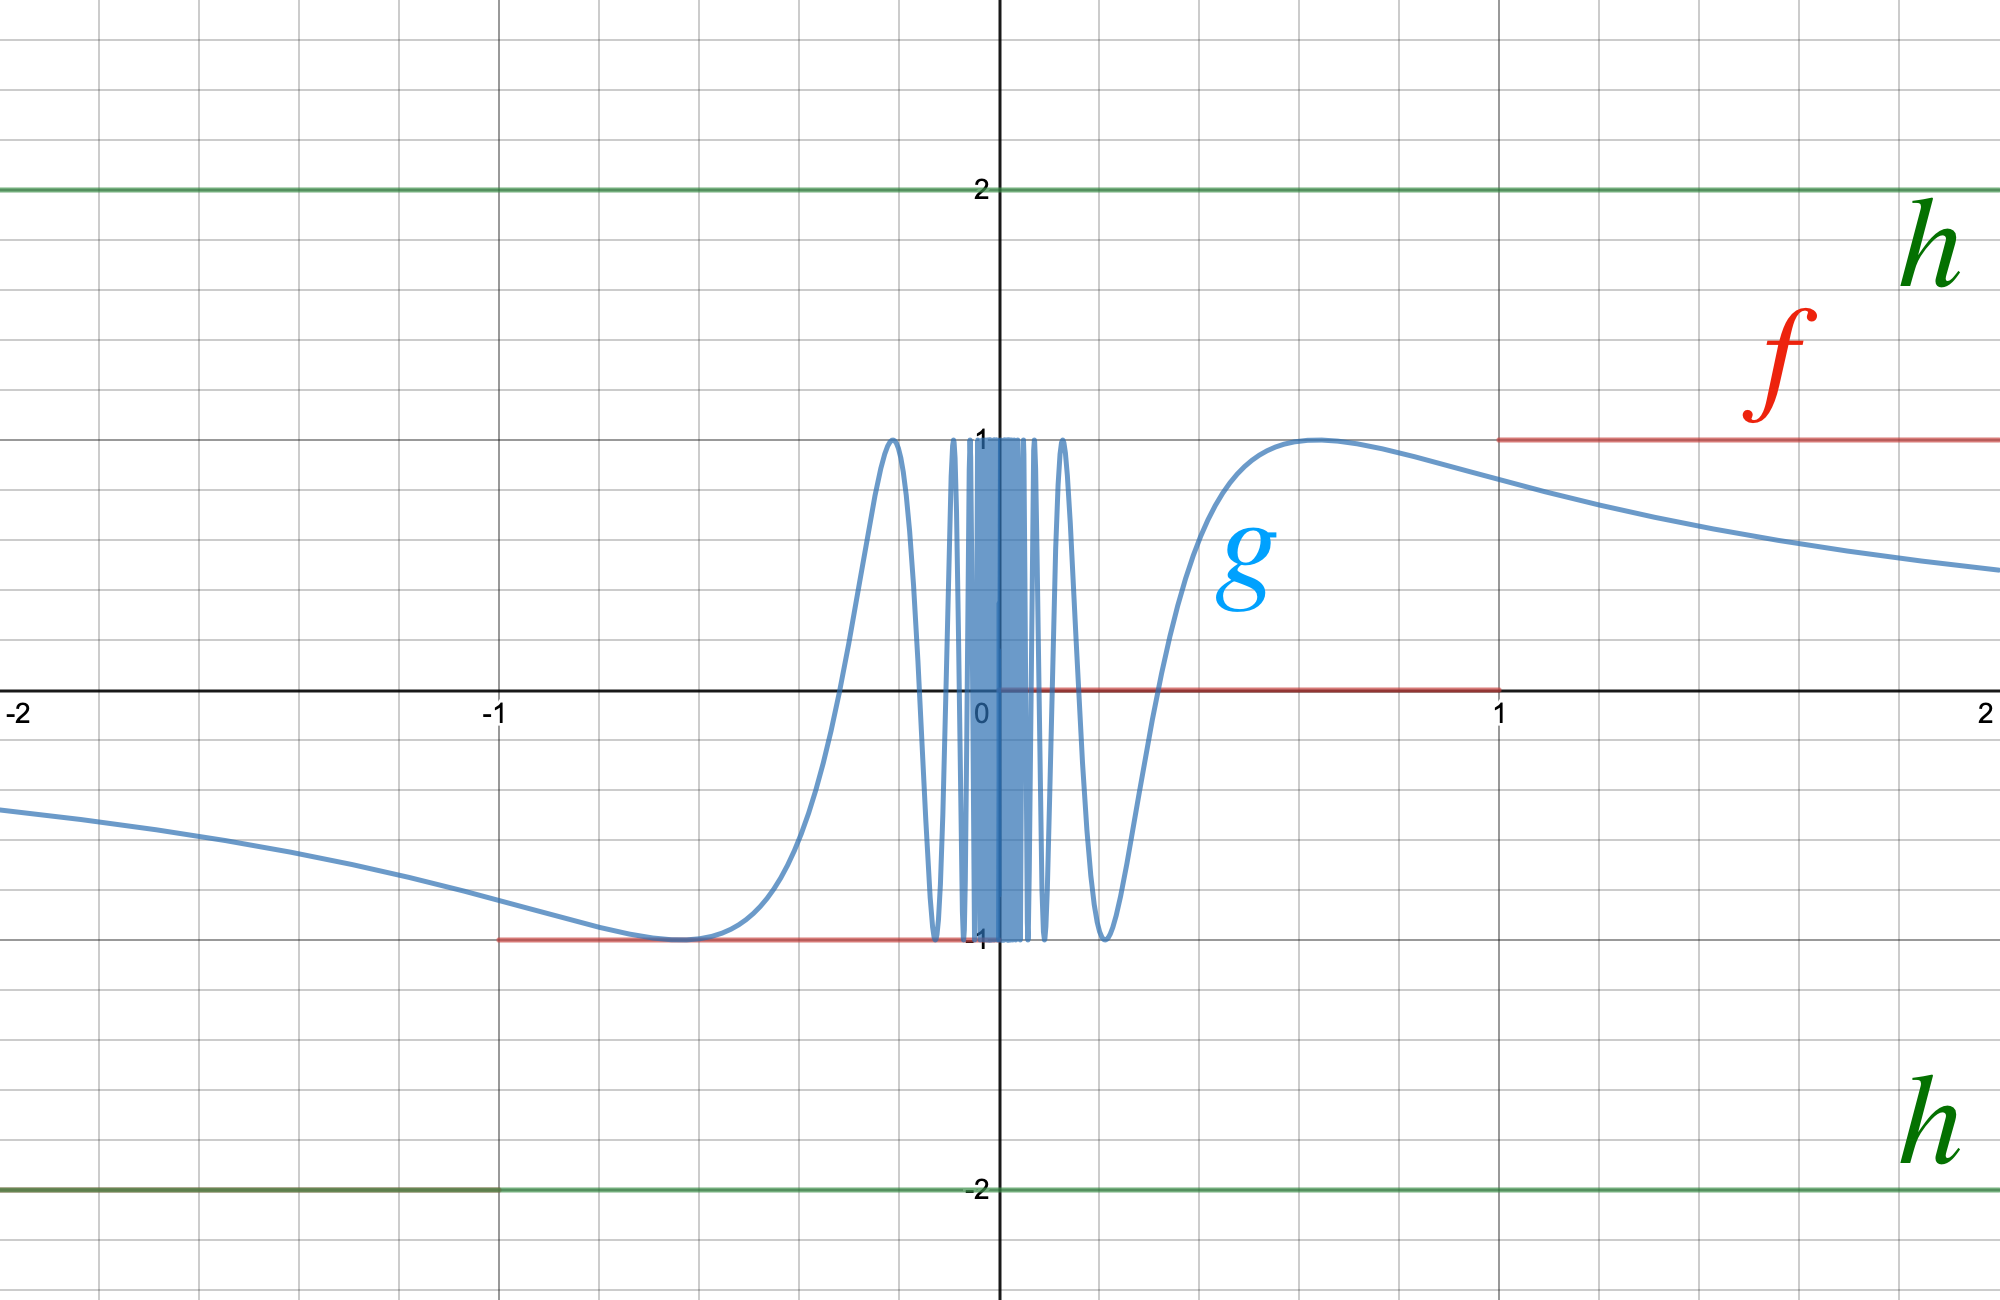
\includegraphics[width=8cm]{pic/DiscontFct.png}
\anngraphics{8cm}{pic/DiscontFct.png}{The graphs of the three discontinuous
functions f (jumping), g (oscillating faster) and h (seemingly two lines)}
\end{center}
\caption{Some discontinuous functions}
\label{figdiscont}
\end{figure}

Our definition of functions however allows for {\em arbitrary} functions, such as the
following ones (Figure~\ref{figdiscont}):
\begin{eqnarray*}
f\colon\R\to\R&,& x\mapsto \lfloor x\rfloor\qquad\mbox{Round down to integer}\\
g\colon\R\to\R&,& x\mapsto
\left\{\begin{array}{ll}
\sin(1/x)&x\not=0\\
1&x=0\\
\end{array}
\right.\\
h\colon\R\to\R&,& x\mapsto
\left\{\begin{array}{ll}
3&x\in\Q\\
-3&x\not\in\Q\\
\end{array}
\right.
\end{eqnarray*}
If we investigate the function $f$ around $1/2$, there is no way to see that it jumps at
0 and at 1. Similarly, why is the value of $g$ at $0$ one (and not zero or $-1$, or
something in between). And we can't even look fine enough to decide from the graph that
$h$ is a function.

Instead, we want that the graph of the function is smooth, that is that we get close to
a point $x$, we can predict the function value $f(x)$. Getting closer will ultimately
give a better approximation.

Formally, we define a function $f\colon\R\to\R$ to be~\defini{continuous} at a point $x_0$
(otherwise: \defini{discontinuous}) if
\begin{quote}
The limit $\displaystyle\lim_{x\to x_0} f(x)$ exists and is equal to the
function value $f(x_0)$.
\end{quote}

If the function is continuous at every point $x_0$, we simply call it continuous (without
``at'').

We see for example that the ``rounding down''
function $f(x)=\lfloor x\rfloor$  is not continuous at $1$,
since the sequence $a_i=1-1/i$ has $\lim_{i\to\infty} a_i=1$, but
$f(a_i)=f(1-1/i)=\lfloor 1-1/i\rfloor=0$, and thus $\lim_{i\to\infty}
f(a_i)=0\not=1=f(1)$.
\medskip

Informally, a function is continuous, if small changes in the argument imply small
changes in the value -- that is we can approximate the function value at $x_0$ by the
function values at numbers close to $x_0$. For the graph of the function
this means that it may not have any jumps, nor start wild oscillations, but
should be followed easily with a pencil. Most functions you will encounter
(that do not jump) are likely to be continuous.

To show formally that a function is continuous, using the definition, can be
hard.  We therefore do not investigate
this further in this class\mynote{There is a criterion that is used in the Calculus class for mathematicians
that formalizes the ``close approximation'' idea, but we do not need it here}. Instead
we study what continuity is good for.

\subsection{Some continuous functions}

Many functions you know from school are continuous. And due to the laws of
limits, it is not just these functions, but also functions composed by
arithmetic operations (as long as a denominator does not become zero), and
also compositions of such functions:

\begin{itemize}
\item Nonnegative powers of $x$: $x^a$ for $a\in\R$. This includes the constant function
$x^0$.
\item Thus also polynomials and (as long as the denominator is nonzero) rational
functions.
\item Trigonometric functions $\sin(x)$, $\cos(x)$, and $\tan(x)=\sin(x)/\cos(x)$ (when
the denominator is nonzero).
\item Inverse trigonometric functions (Note that $\arcsin$ and $\arccos$ are only defined
on the domain $\{-1\ldots 1\}$.
\item The exponential function $\exp(x)=e^x$ and (for positive $x$) its
inverse the natural logarithm $\log(x)=\ln(x)$. (All logarithms in this
course without a specific basis are natural logarithms.)
\end{itemize}

The definition of some of these functions (such as $\sin(x)$ as measurement
on a triangle in a circle) given in
school is not amenable to easy computation, we will see later
\pointer{sectaylors} how this can be done.

\section{Why Care About Continuity}
\label{secwhycont}

The first use of continuity is that it makes approximation meaningful. We can work, for
example, with numerical approximations of $x$ values, and trust that the function value
$f(x)$ will not differ too much from $f(x_0)$ if $x$ is an approximation of $x_0$.

A consequence of this is that we can ``control'' the function values. If we want to find
$x$ to achieve a particular function value $f(x)$, we can do so by iterative
approximation. On the other hand, the situation that small changes in the input could
produce (arbitrary) large changes in the output is close to the definition of chaos.
\smallskip

A consequence of this property is the following statement:
\begin{figure}
\begin{center}
%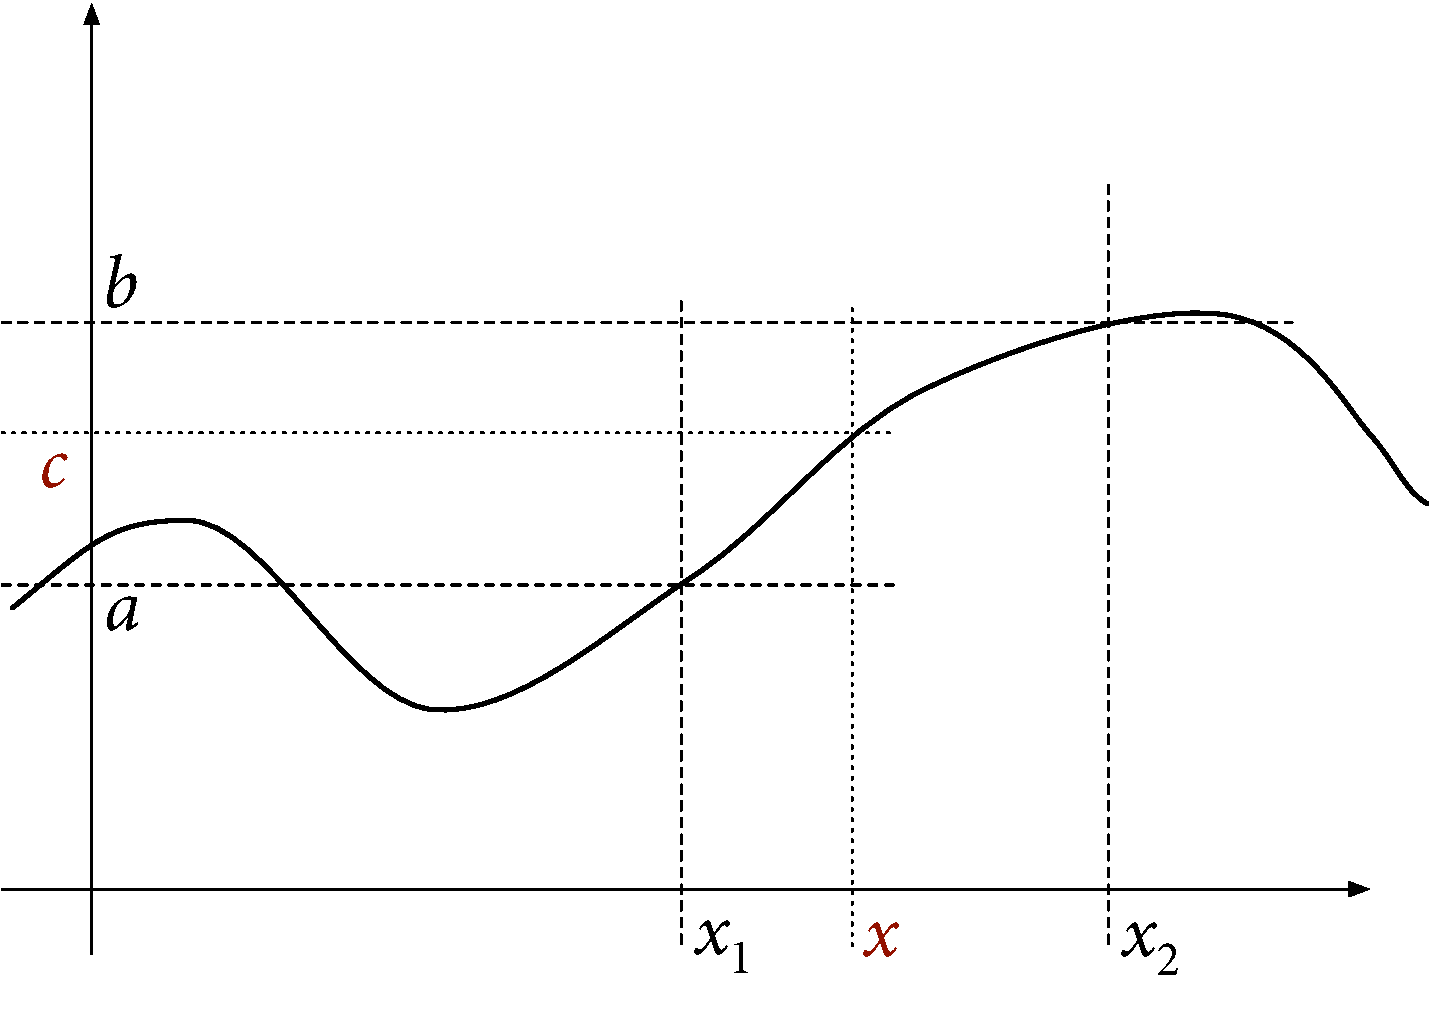
\includegraphics[width=6cm]{pic/IntermedThm.pdf}
\anngraphics{6cm}{pic/IntermedThm.png}{The Intermediate Value Theorem
illustrated on a coordinate plane. The point $(x, c)$ exists between the
points $(x_1, a)$ and $(x_2, b)$ on a curving, continuous graph.}
\end{center}
\caption{The intermediate Value Theorem}
\label{figivt}
\end{figure}
\begin{thm}[Intermediate Value Theorem]
Let $f\colon\R\to\R$ be a continuous function and $x_1<x_2\in\R$ with $f(x_1)=a$ and
$f(x_2)=b$. Let $c$ be a number between $a$ and $b$. Then there exists $x_1\le x\le x_2$
such that $f(x)=c$ (Figure~\ref{figivt}).
\end{thm}

We can use this theorem to find $x$ for a particular $f(x)$-value. Most frequently this
is done to find $x$, such that $f(x)=0$. The method is called \defini{halving
intervals} or \defini{bisection} method.
\begin{enumerate}
\item
Start with $s,t\in\R$ such that $f(s)<0$ and $f(t)>0$. (Or vice versa: $f(s)>0$ and
$f(t)<0$.)
\item Let $m=\frac{s+t}{2}$ be the midpoint of the interval. If $f(m)=0$ and
stop. Otherwise:
\item If $f(s)$ and $f(m)$ have the same sign (positive or negative) replace $s$ by $m$.
Otherwise replace $t$ by $m$ (since $f(m)$ and $f(t)$ have the same sign).
\item If $\sz{t-s}$ is not small enough (to the approximation quality we want), go to
step 2.
\end{enumerate}
In each step of the algorithm, the length of the interval from $s$ to $t$ halves, and
the desired $x$ value must lie in the interval. We can repeat until $s$ and $t$
approximate this $x$ sufficiently well.

For example, consider the function $f(x)=\sin(x)$. We want to approximate the number
$\pi$, knowing\mynote{We measure the angle of a full circle as $2\pi$}
that $f(\pi)=0$. We start with $s=2$ and $t=4$, since we know that
$2<\pi<4$. We now iterate, setting $m=(2+4)/2=3$ and calculate $f(3)$, which is
positive. Thus we replace $s$ by $3$ and iterate. The following table shows the
further iterations (with underlined numbers indicating the end point that was replaced
by $m$ in each step).
After 20 iterations, the length of the interval has become $2/2^{20}\sim 10^{-6}$. This
agrees with the fact that we gain a further correct digit every
$\log_2(10)\sim 3.3219$ steps and thus should expect $20/3.3219=6$ correct digits in the result,
approximating $\pi$ as $3.141593$ (versus the correct\mynote{Count the digits in each
word in the sentence {\em
How I want a drink, alcoholic of course, after the heavy chapters involving quantum
mechanics}.} $3.1415926\ldots$).
\begin{center}
\begin{tabular}{@{}rl@{\,\,\,\,}l@{\,\,\,\,}l@{\,\,\,\,}l@{\,\,\,\,}l@{\,\,\,\,}l@{\,\,\,\,}l@{}}
\#&$s$&$t$&$\sz{t-s}$&$f(s)$&$f(t)$&$m=\frac{s+t}{2}$&$f(m)$\\
0&2&4&2&0.909297&-0.756802&3&0.141120\\
1&\underline{3}&4&1&0.141120&-0.756802&3.5&-0.350783\\
2&3&\underline{3.5}&0.5&0.141120&-0.350783&3.25&-0.108195\\
3&3&\underline{3.25}&0.25&0.141120&-0.108195&3.125&0.016592\\
4&\underline{3.125}&3.25&0.125&0.016592&-0.108195&3.1875&-0.045891\\
5&3.125&\underline{3.1875}&0.0625&0.016592&-0.045891&3.156250&-0.014657\\
6&3.125&\underline{3.15625}&0.03125&0.016592&-0.014657&3.140625&0.000968\\
7&\underline{3.140625}&3.156250&0.015625&0.000968&-0.014657&3.148438&-0.006845\\
8&3.140625&\underline{3.148438}&0.007813&0.000968&-0.006845&3.144531&-0.002939\\
9&3.140625&\underline{3.144531}&0.003906&0.000968&-0.002939&3.142578&-0.000985\\
10&3.140625&\underline{3.142578}&0.001953&0.000968&-0.000985&3.141602&-0.000009\\
11&3.140625&\underline{3.141602}&0.000977&0.000968&-0.000009&3.141113&0.000479\\
12&\underline{3.141113}&3.141602&0.000488&0.000479&-0.000009&3.141357&0.000235\\
13&\underline{3.141357}&3.141602&0.000244&0.000235&-0.000009&3.141479&0.000113\\
14&\underline{3.141479}&3.141602&0.000122&0.000113&-0.000009&3.141541&0.000052\\
15&\underline{3.141541}&3.141602&0.000061&0.000052&-0.000009&3.141571&0.000022\\
16&\underline{3.141571}&3.141602&0.000031&0.000022&-0.000009&3.141586&0.000006\\
17&\underline{3.141586}&3.141602&0.000015&0.000006&-0.000009&3.141594&-0.000001\\
18&3.141586&\underline{3.141594}&0.000008&0.000006&-0.000001&3.141590&0.000003\\
19&\underline{3.141590}&3.141594&0.000004&0.000003&-0.000001&3.141592&0.000001\\
20&\underline{3.141592}&3.141594&0.000002&0.000001&-0.000001&3.141593&-0.000000\\
\end{tabular}
\end{center}
Such a process of halving intervals can be implemented easily. It however
takes a while to get a good approximation, which is why we will see a better
method in a later chapter~\pointer{secnewton}.

\section{Partial Sums and Derived Sequences}

Before defining derivatives properly, let us look at an example of change
that happens at discrete intervals, and how function values and change are
related.


Imagine
the ledger of a business that lists every day the sum of income minus expenses
(let's call it the \defini{flow}), and the total money held by the business:

\begin{center}
\begin{tabular}{rrr}
Day&Income-Expenses&Money held\\
\hline
0& - &0\\
1&893&893\\
2&70&963\\
3&992&1955\\
4&682&2637\\
5&115&2752\\
6&215&2967\\
7&-497&2470\\
8&-246&2224\\
9&252&2476\\
10&-301&2175\\
\end{tabular}
\end{center}

Going through the columns, we get two sequences, both indexed by the first
column.  The first sequence, which we shall call $a_i$ is the daily flow.
The second sequence, let's call it $b_i$, is the money held by the business.
Is there a relation between the two columns?

Of course. Assuming we started with $0$ money held, the money held on the end of day
$i$ is the sum of the flow of days $1$ to $i$. We write this as
$$b_i=a_1+a_2+a_3+\cdots+ a_{i-1}+a_i=\sum_{j=1}^i a_j$$
and have that the $b_i$ are the *partial sums* over the sequence $a_i$.

Can we do the same thing backwards? Surely -- solving for $a_i$ finds that
$$a_i=\sum_{j=1}^ia_i-\sum_{j=1}^{i-1}a_i=b_i-b_{i-1}.$$

The two sequences are thus ``related" in that each sequence completely
determines the other one and vice versa. We shall call the sequence $\{a_i\}$
the \defini{derivative sequence} of the sequence $\{b_i\}$ and the sequence
$\{b_i\}$
an \defini{antiderivative} or an
\defini{indefinite integral} of $\{a_i\}$.

Calculus is about studying such a correspondence between functions defined on
(e.g.) the real numbers, while sequences are functions defined on the
positive integers.

Before going there, let us look at a few ways how this correspondence plays
out and helps us with determining information.
First, imagine we would have started not at 0 but with some money in the
bank, say 1000 currency units. Then the ledger would have looked almost the
same, but for the last column being increased by 1000:

\begin{center}
\begin{tabular}{rrr}
Day&Income-Expenses&Money held\\
\hline
0& - &1000\\
1&893&1893\\
2&70&1963\\
3&992&2955\\
4&682&3637\\
5&115&3752\\
6&215&3967\\
7&-497&3470\\
8&-246&3224\\
9&252&3476\\
10&-301&3175\\
\end{tabular}
\end{center}

Denote the sequence given by the third column in this ledger by $c_i$. We
note that $c_i$ is built from the *same changes* as $b_i$ is. Thus $a_i$ is
also the derivative of $c_i$ and $c_i$ is an integral of $a_i$. (That is why
we said ``an integral'' and not ``the integral''.) It is not hard to see that
there are many more antiderivatives (namely, different starting values in the
bank), but that any two antiderivatives simply differ by a constant (namely
the difference of their starting account values).

If we care about the flow over a number of days, say from day 4 to day 7
(inclusively), we need to add up the flows of these three days:
$$a_4+a_5+a_6+a_7=\sum_{j=4}^7 a_j.$$
Using the sum notation, we see that this multi-day flow difference also can
be expressed as a difference of values of an antiderivative over multiple
days, we have that
$$\sum_{j=4}^7 a_j=(\sum_{j=1}^7 a_j)-(\sum_{j=1}^3 a_j)=b_7-b_3=c_7-c_3.$$
Here $7$ is the time when the counting ends (the evening of day 7) and $3$
the time when it starts (the evening of day $3$ as giving the same amount as
on the morning of day $4$ which is not listed separately in the ledger.)

This difference formula will hold for whatever antiderivative we are
choosing. This holds, because the starting account value has no impact on
the flow over the four days we are measuring. Thus antiderivatives (more
specifically the {\em difference} of the values of antiderivatives between a
start and an end point, which will be called a \defini{definite integral}.)
We will encounter this easy idea later again under the name of
``Fundamental Theorem of Calculus''.
\medskip

We have seen that an antiderivative helps with summing up changes over a
period. But what can derivatives be used for? To illustrate this, look at
a different sequence $\{b_i\}$ (starting with $b_0$) whose changes are smaller, but which we tabulate
over a longer range:
\begin{eqnarray*}
&&
 0, 8, 15, 21, 24, 26, 28, 26, 25, 23, 21, 19, 18, 16, 15, 14, 13, 14, 15,
  16, 18, 20, 22, 25,\\
 &&\qquad 28, 31, 34, 37, 40, 43, 46, 48, 50, 51, 52, 53, 52, 51,
  49, 48, 45, 42, 40, 36, 33,\\
  &&\qquad 31, 28, 27, 26, 27, 30
\end{eqnarray*}
We get a sequence of changes $\{a_i\}$ (starting with $a_1$) as
$a_i=b_i-b_{i-1}$:
\begin{eqnarray*}
&&
7, 6, 3, 2, 2, -2, -1, -2, -2, -2, -1, -2, -1, -1, -1, 1, 1, 1, 2
\end{eqnarray*}
The values of both sequences are depicted (with points connected) in
Figure~\ref{figpythder}.

\begin{figure}
\begin{center}
%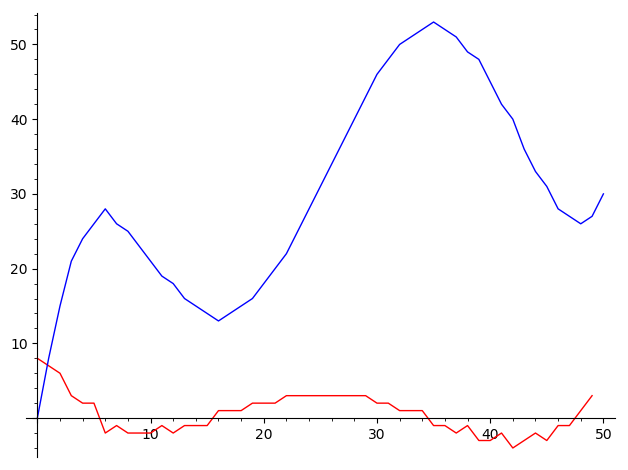
\includegraphics[width=8cm]{pic/pythder.png}
\anngraphics{8cm}{pic/pythder.png}{The values obtained from the sequence of
changes, ${a_i}$, and the values of the original sequence ${b_i}$, plotted
on a coordinate plane.}
\end{center}
\caption{A sequence and its derivative}
\label{figpythder}
\end{figure}

An obvious question one can ask for such a sequence $b_i$ is for what the
maximum and minimum (largest and smallest) values over the investigated
period are.
(In the previous example these would have been the lowest and the highest
worth of the business.) We mark the areas where the function is (locally,
that is in relation to its neighbors) maximal or minimal in
Figure~\ref{figpythder2}.

\begin{figure}
\begin{center}
%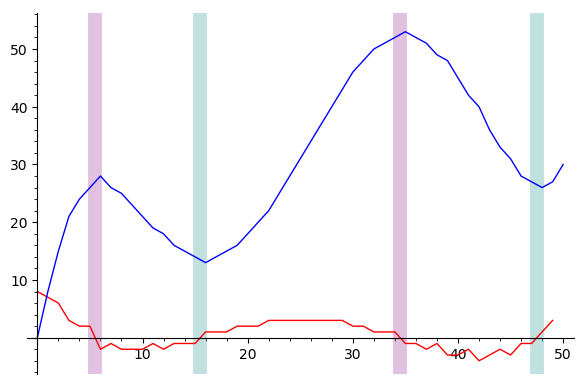
\includegraphics[width=8cm]{pic/pythder2.png}
\anngraphics{8cm}{pic/pythder2.png}{On the coordinate plane, the maximum
values on the graph of ${b_i}$ coincide with places where the graph of
${a_i}$ intersect the x-axis. The same is true for minimum values of
${b_i}$.}
\end{center}
\caption{Maxima and Minima}
\label{figpythder2}
\end{figure}

We note that at these index values (for which the function $b_n$ is maximal,
respectively minimal), which are aligned along the $x$-axis, the derivative
is zero. (An eagle-eyed reader might notice that we are slightly cheating
here: Since we sum up the values of the derivative, the maximum happens at
the $x$-value plus 1, and our derivatives are only close to zero. This will
be resolved later when we will decrease the step-width more and more.)

Furthermore, at an index $i$, where $b_i$ has minimum value, the derivative
$a_i$ changes from being negative to being positive. And at the index $i$
where $b_i$ has maximum value, the derivative changes sign from positive to
negative.  The reason for this is easily understood. To be a maximum value
(say),at index $i$m the values must have grown in step $i$ (that is the
derivative is positive at $i$), as otherwise the value cannot be larger than
other different ones. But if the derivative did not become negative at
$i+1$, the function would have been growing even further.

Thus, if we look at all places where the derivative changes from positive to
negative we see that these are exactly the *local maxima*, that is the
places where the function is larger than in the neighborhood (with the same
argument about growing before but not after).

A similar kind of argument can be made for local minima.

Finding indices where the derivative is (close to) zero is easy. The
derivative thus allows us to find maxima or minima (which are harder to
find).
\smallskip

This is a further indication that the concept of a derivative is a useful
concept, and we will spend most of the remainder of the class studying
derivatives and antiderivatives and their consequences.

\section{Aliasing}

The concept of summing up changes is rather basic, and the reader might
wonder what else there could be to Calculus. One fundamental issue is that
the prior example had a natural step-width (the day), while this is not true
for many other situations. Indeed, results might be fundamentally wrong if
we impose an artificial step-width. This phenomenon goes under the name of
\defini{aliasing} and also can occur when digitizing pictures or sound
signals. In this section (which is not required later on) we illustrate what
can happen.
\smallskip

Imagine we  have temperatures oscillating as on a typical winter day in
Colorado, with a cold mornings but temperate early afternoons. The red curve
in Figure~\ref{figalias}, left (with the $x$-axis indicating days) shows
how temperature changes over time. Now an alien (who has no concept of an
Earth day) samples the temperature, namely in intervals if $0.8$ days. The
blue dots indicate the measurements. Based on these measured values, one
clearly would expect the temperature to fluctuate periodically in a cycle of
$4$ days, as indicated by the blue curve in Figure~\ref{figalias}, right.
\begin{figure}
\begin{center}
%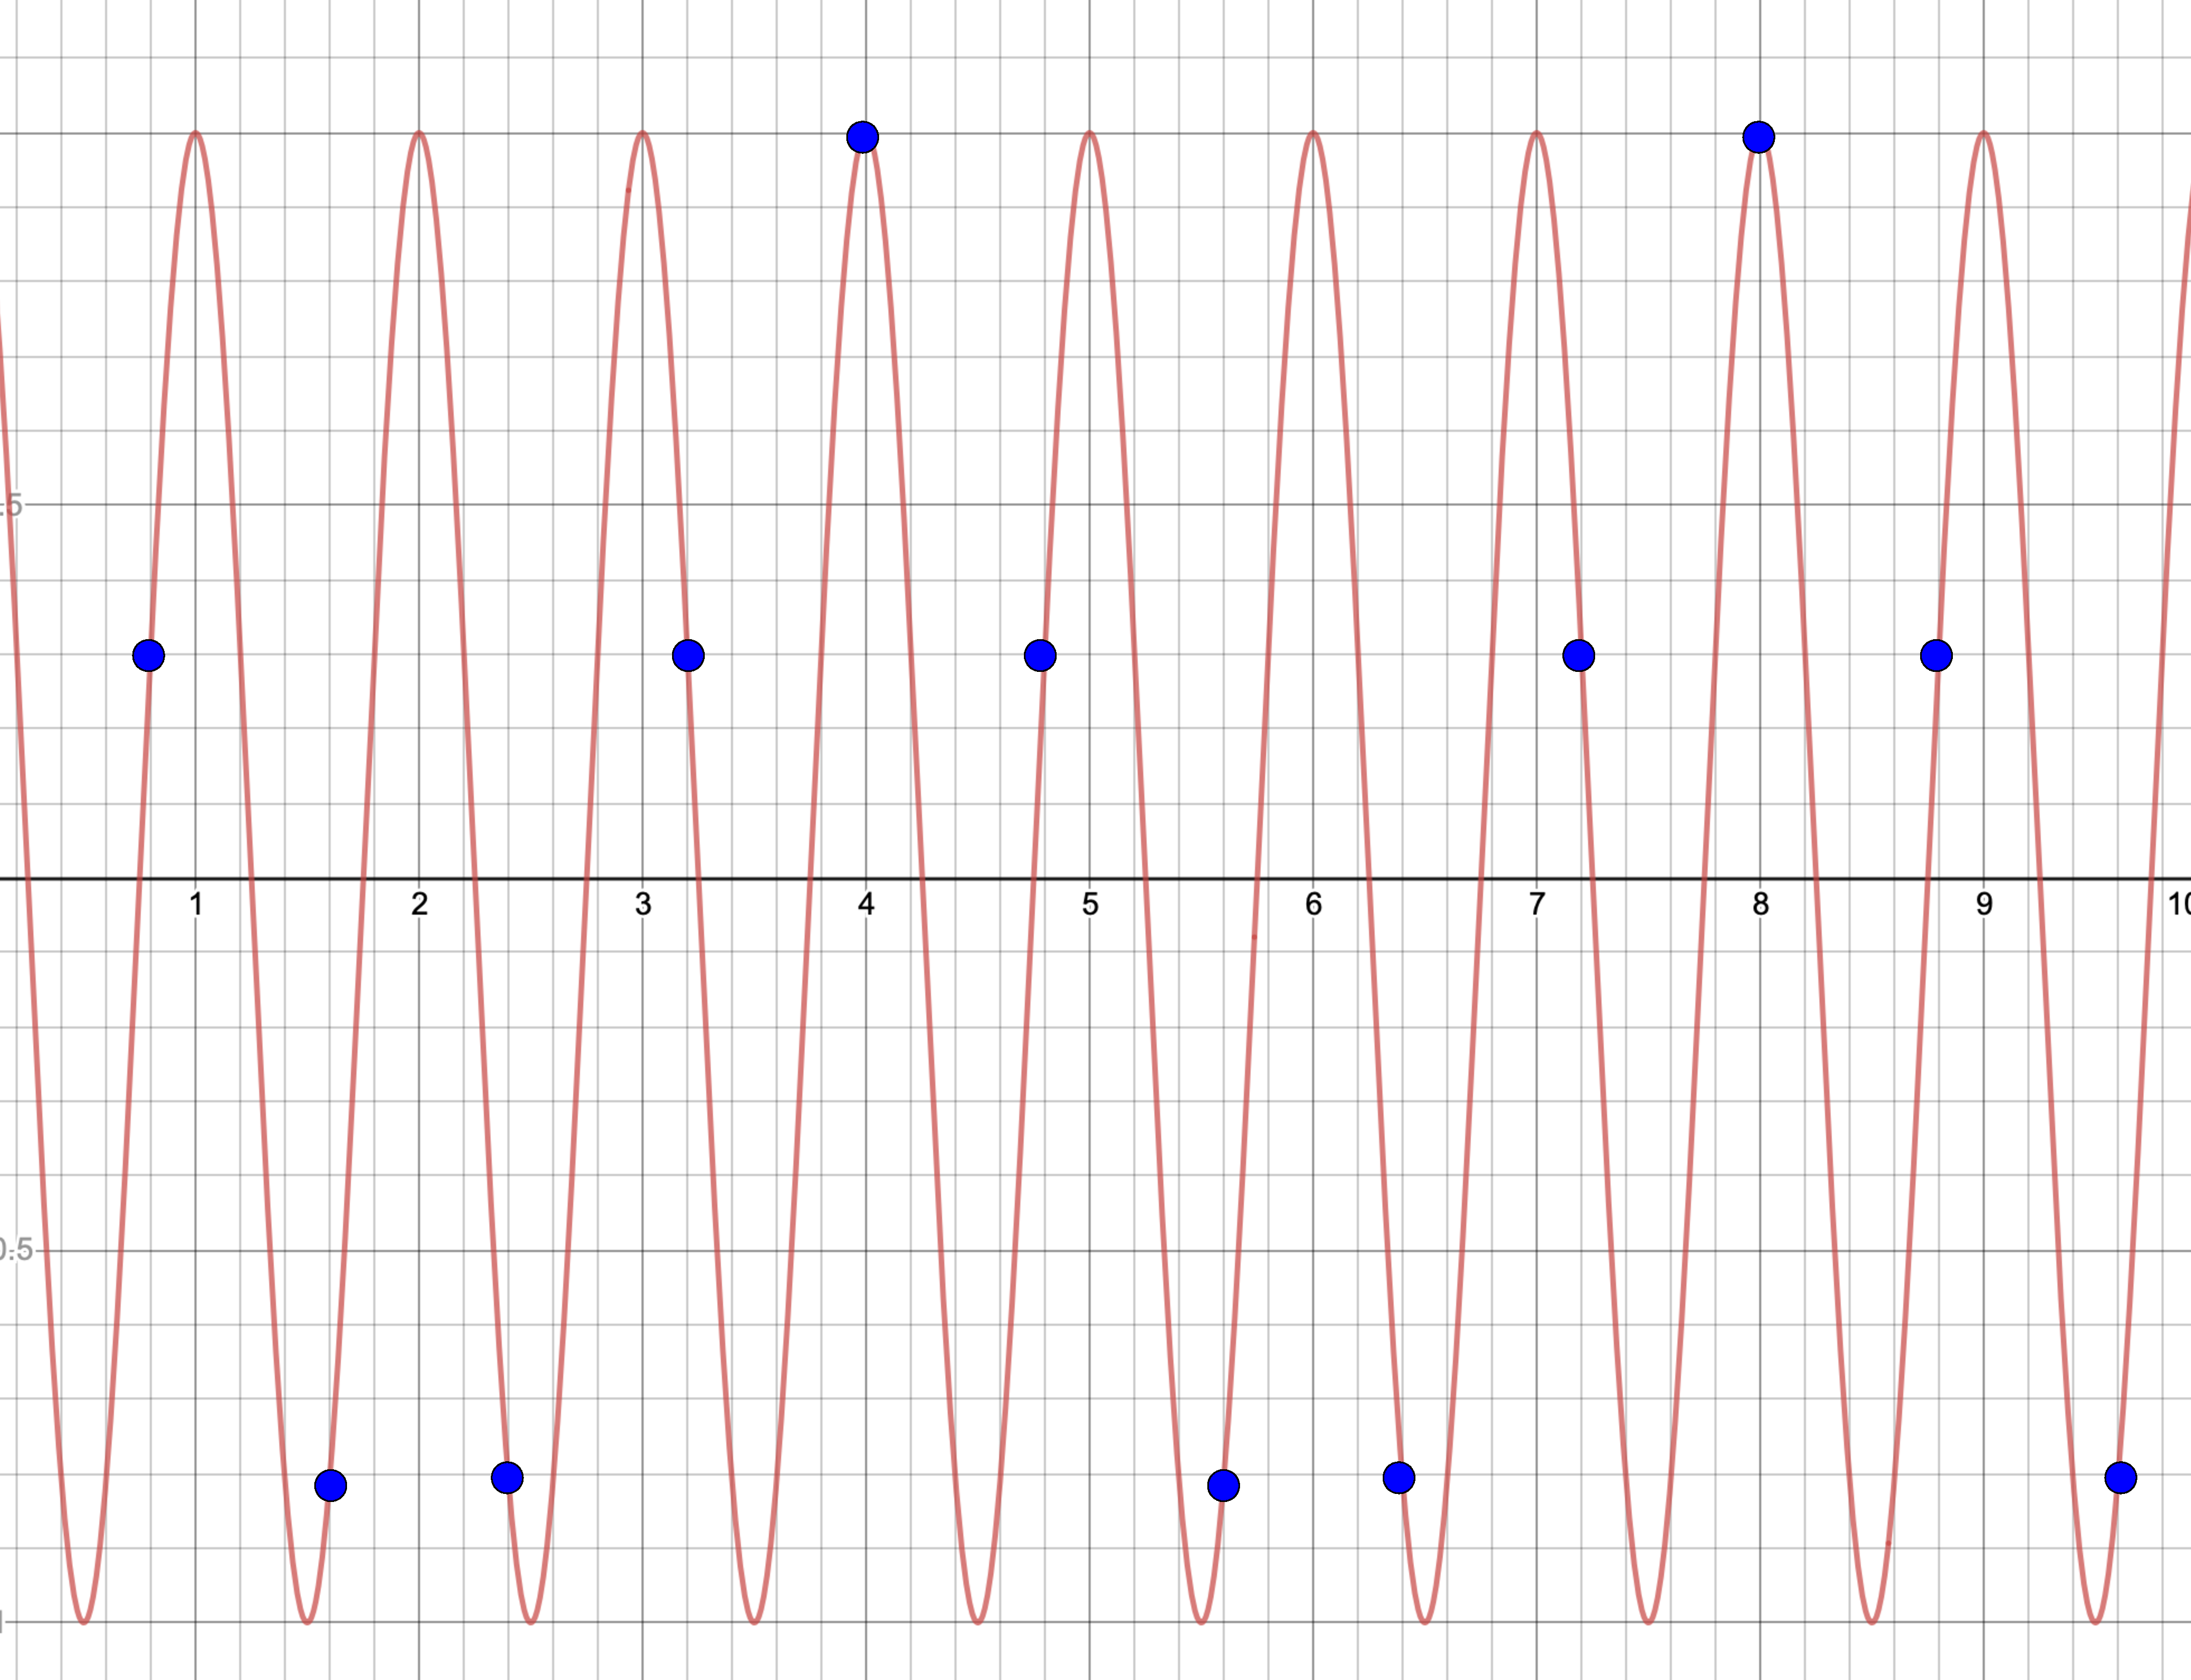
\includegraphics[width=5cm]{pic/Aliasing1.pdf}
\anngraphics{5cm}{pic/Aliasing1.png}{A sinusoidal graph and some sampling
points at regular distances}
\quad
%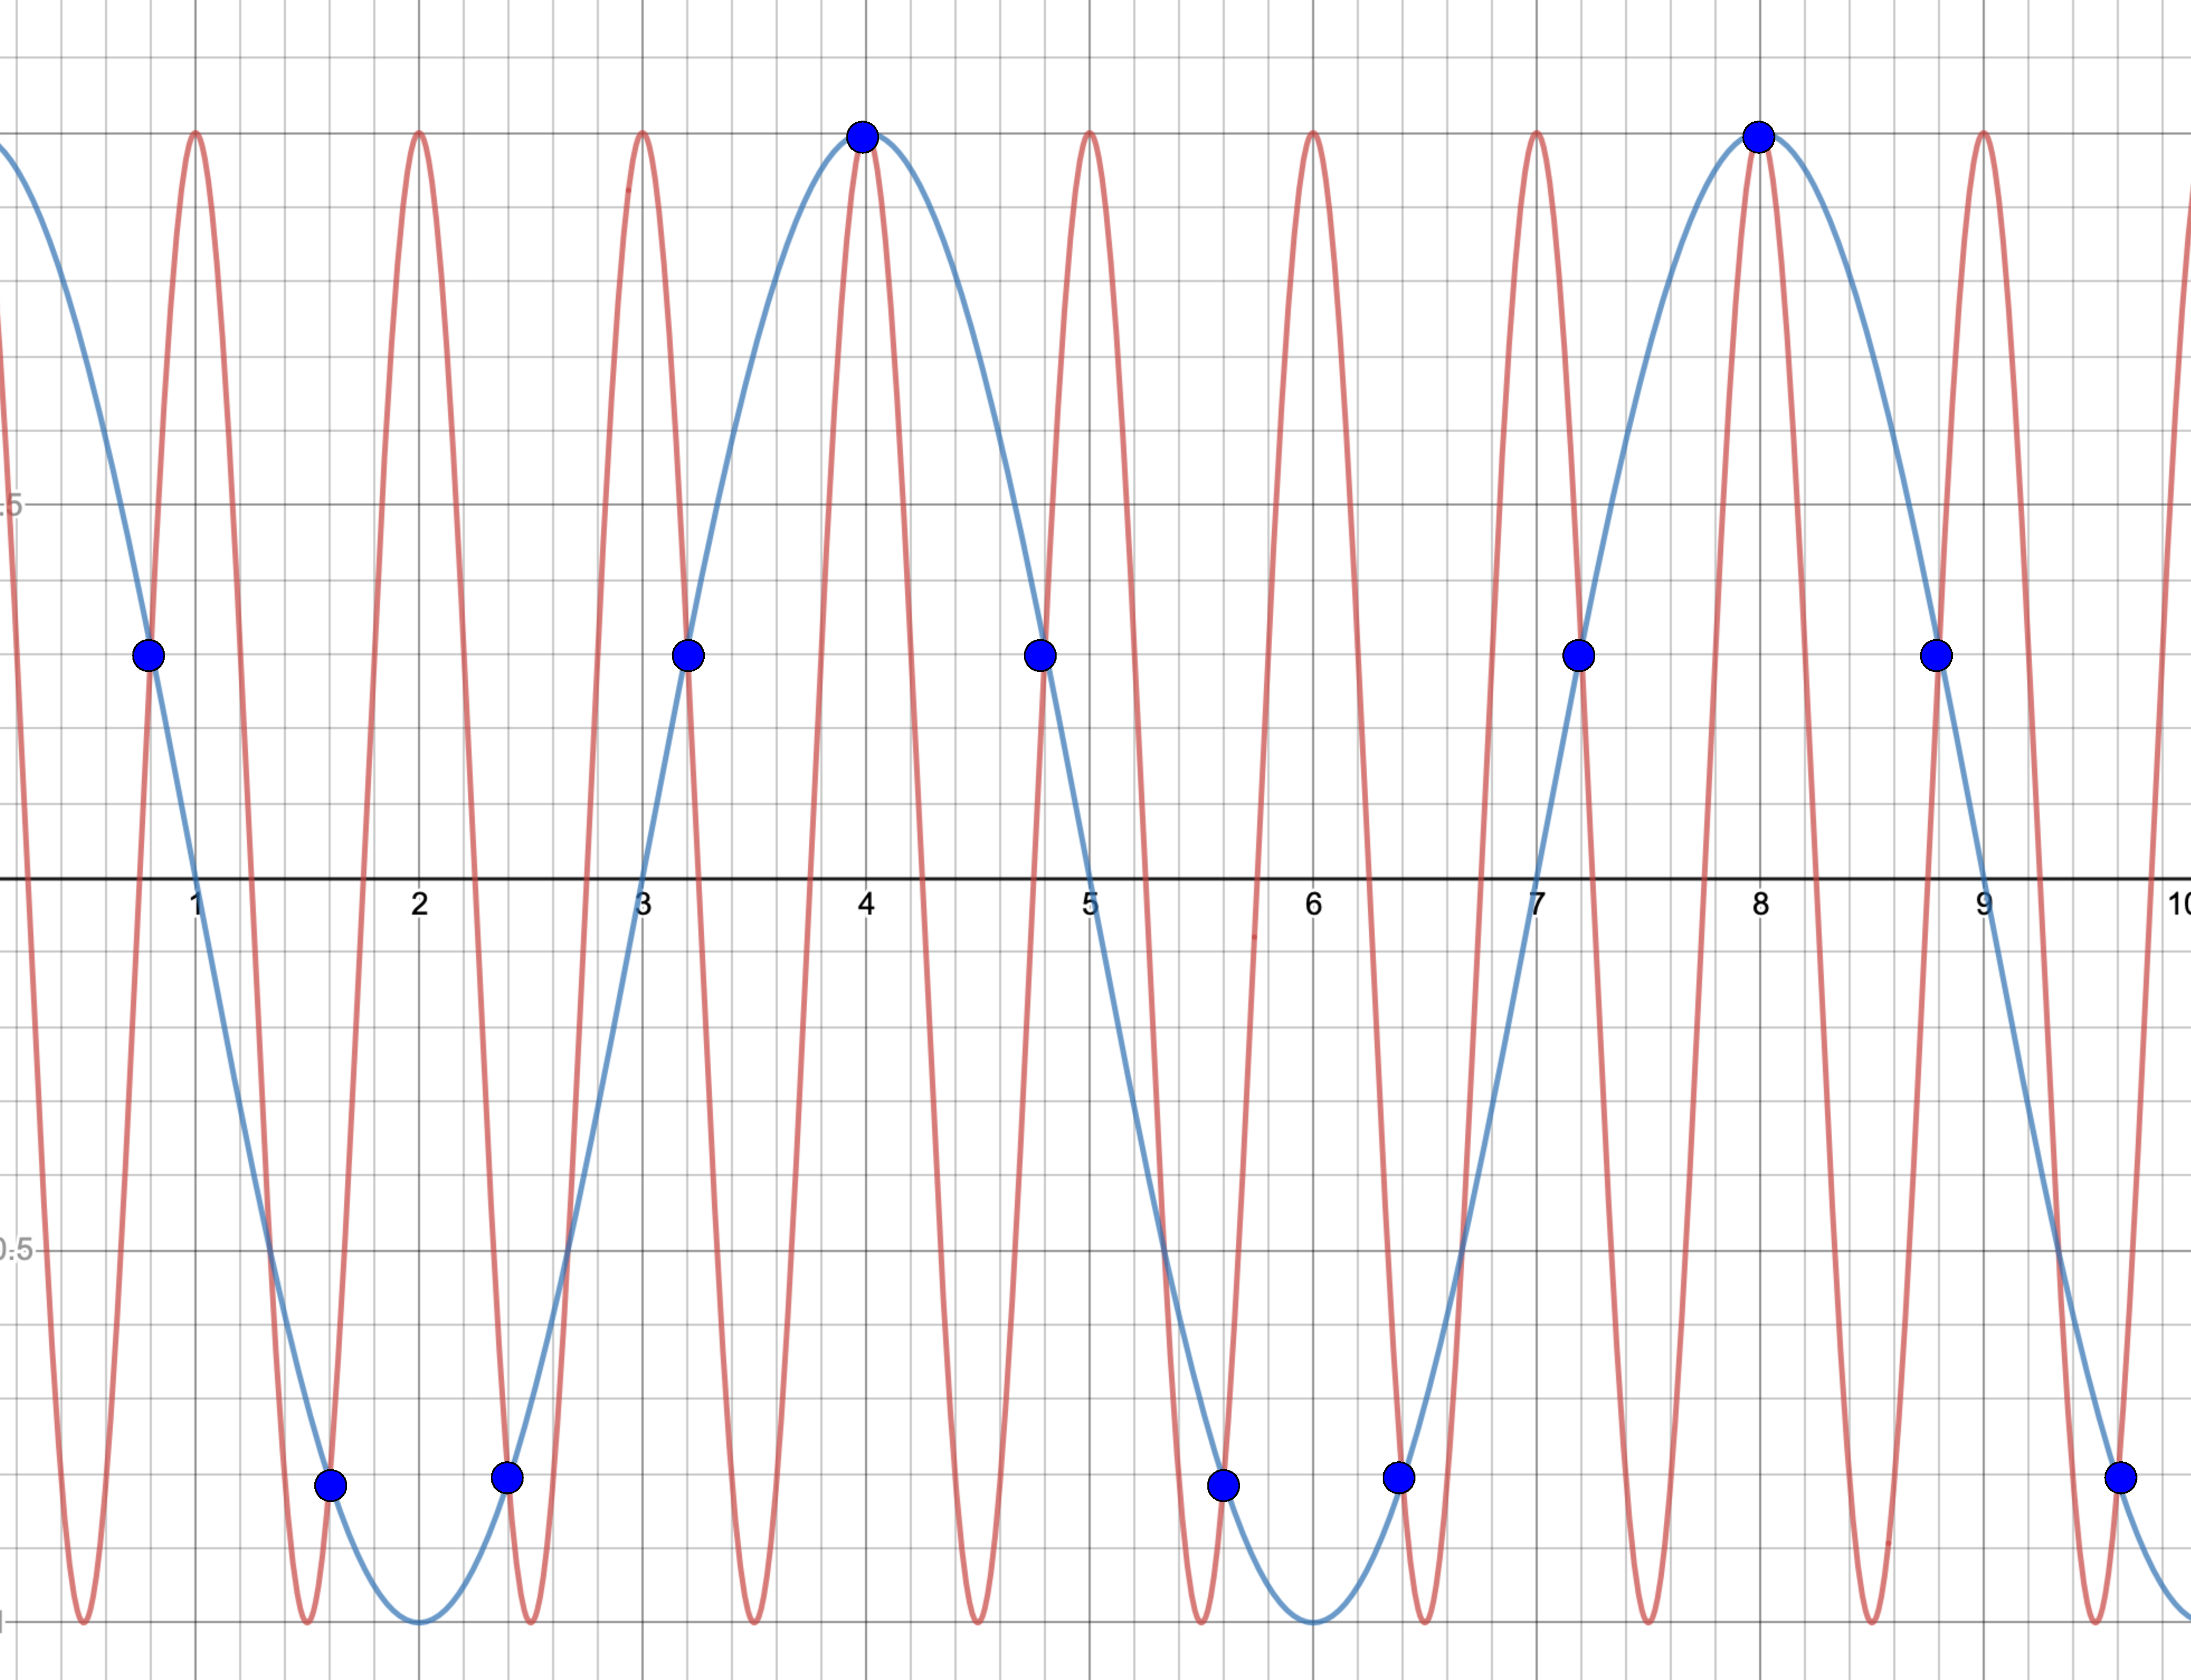
\includegraphics[width=5cm]{pic/Aliasing2.pdf}
\anngraphics{5cm}{pic/Aliasing2.png}{By sampling pieces of data spaced
farther apart, the graph constructed by the alien is much wider and not
reflective of the original, narrowly oscillating graph on the coordinate
plane.}
\end{center}
\caption{Bad sampling leads to aliasing}
\label{figalias}
\end{figure}
Different sample periods will lead to differently bad results (a sample
period of exactly one day would indicate that

The \defini{Nyquist}-\defini{Shannon} sampling theorem in fact shows, that
one needs to sample a periodic signal at at least twice the maximal
frequency (that is twice per period) to be able to detect these frequencies.


The same effect can be seen in so-called \defini{Moir\'e} patterns when
overlaying fabric meshes or when naively reducing the size of a digital
image, as in Figure~\ref{figscreenpic}: When reducing the image by simply
sampling pixels at regular intervals, not only does an underlying regular
grid (from taking a picture off a monitor) become overwhelming, even the
direction of the grid changes! A more sophisticated algorithm instead will
try to keep colors in local areas the same and is able to produce a much
better result (the right image has the same reduced size parameters as the
middle one).
\begin{figure}
\begin{center}
%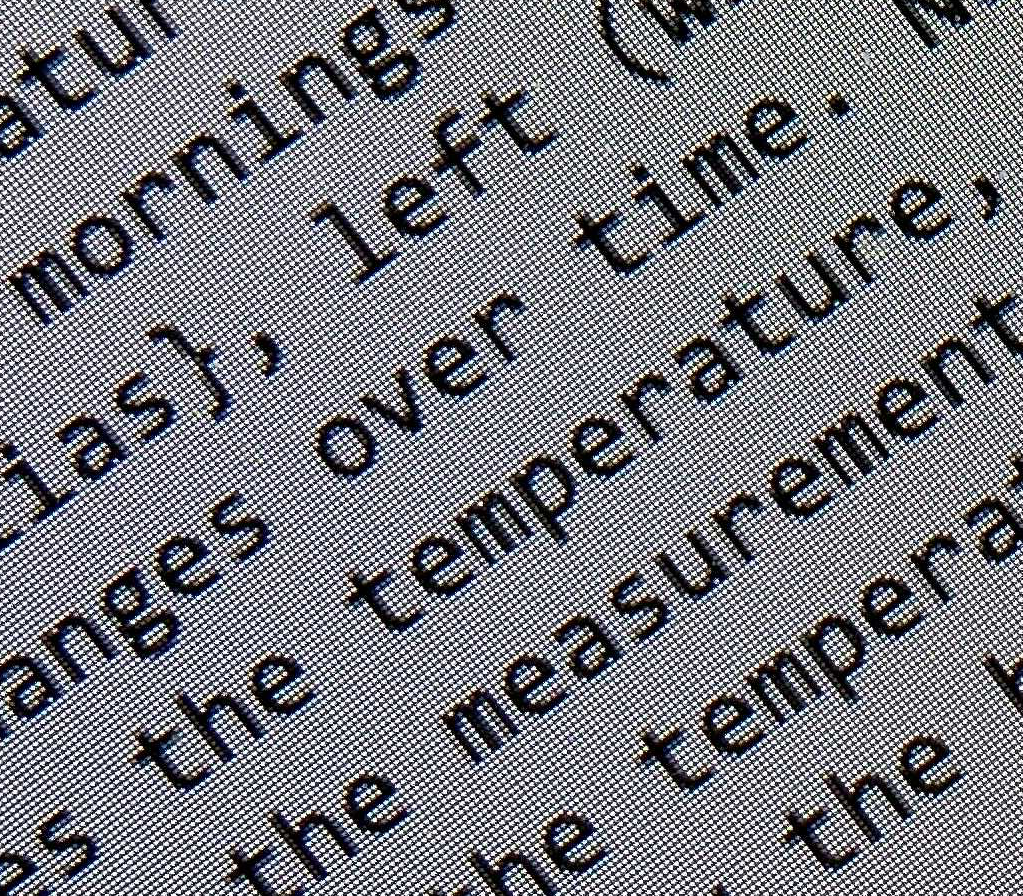
\includegraphics[width=35mm]{pic/screenphoto.png}
\anngraphics{35mm}{pic/screenphoto.png}{A photo taken off a computer
monitor, showing pixes}
\quad
%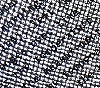
\includegraphics[width=35mm]{pic/screenphoto2.png}
\anngraphics{35mm}{pic/screenphoto2.png}{The picture reduced in size by regular
sampling -- a Moir'e mesh appears and makes the image unintellegible}
\quad
%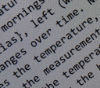
\includegraphics[width=35mm]{pic/screenphoto3.png}
\anngraphics{35mm}{pic/screenphoto3.png}{The picture reduced in size by a
more sophisticated algorithm of a graphics processing program. The relevant
content is still well recognizable, while the regular pixel structure has
been diminished}
\end{center}
\caption{Image reduced by bad and by good algorithm}
\label{figscreenpic}
\end{figure}

\section{The Derivative of a Function}

We have seen that it can be useful to study how the values of a function
change. Let us look at what this means for a function defined on the real
numbers: We could, at a point $x_0$ look how the function changes between
$x_0$ and $x_0+1$ (namely by $f(x_0+1)-f(x_0)$). But there is really no
reason to take a step of $1$. We could similarly look at the change when
taking a step by $2$ or by $\frac{1}{2}$. And of course one would expect the
change to be larger if the step-width becomes larger.

\subsection{Secant Slope}

\begin{figure}
\begin{center}
%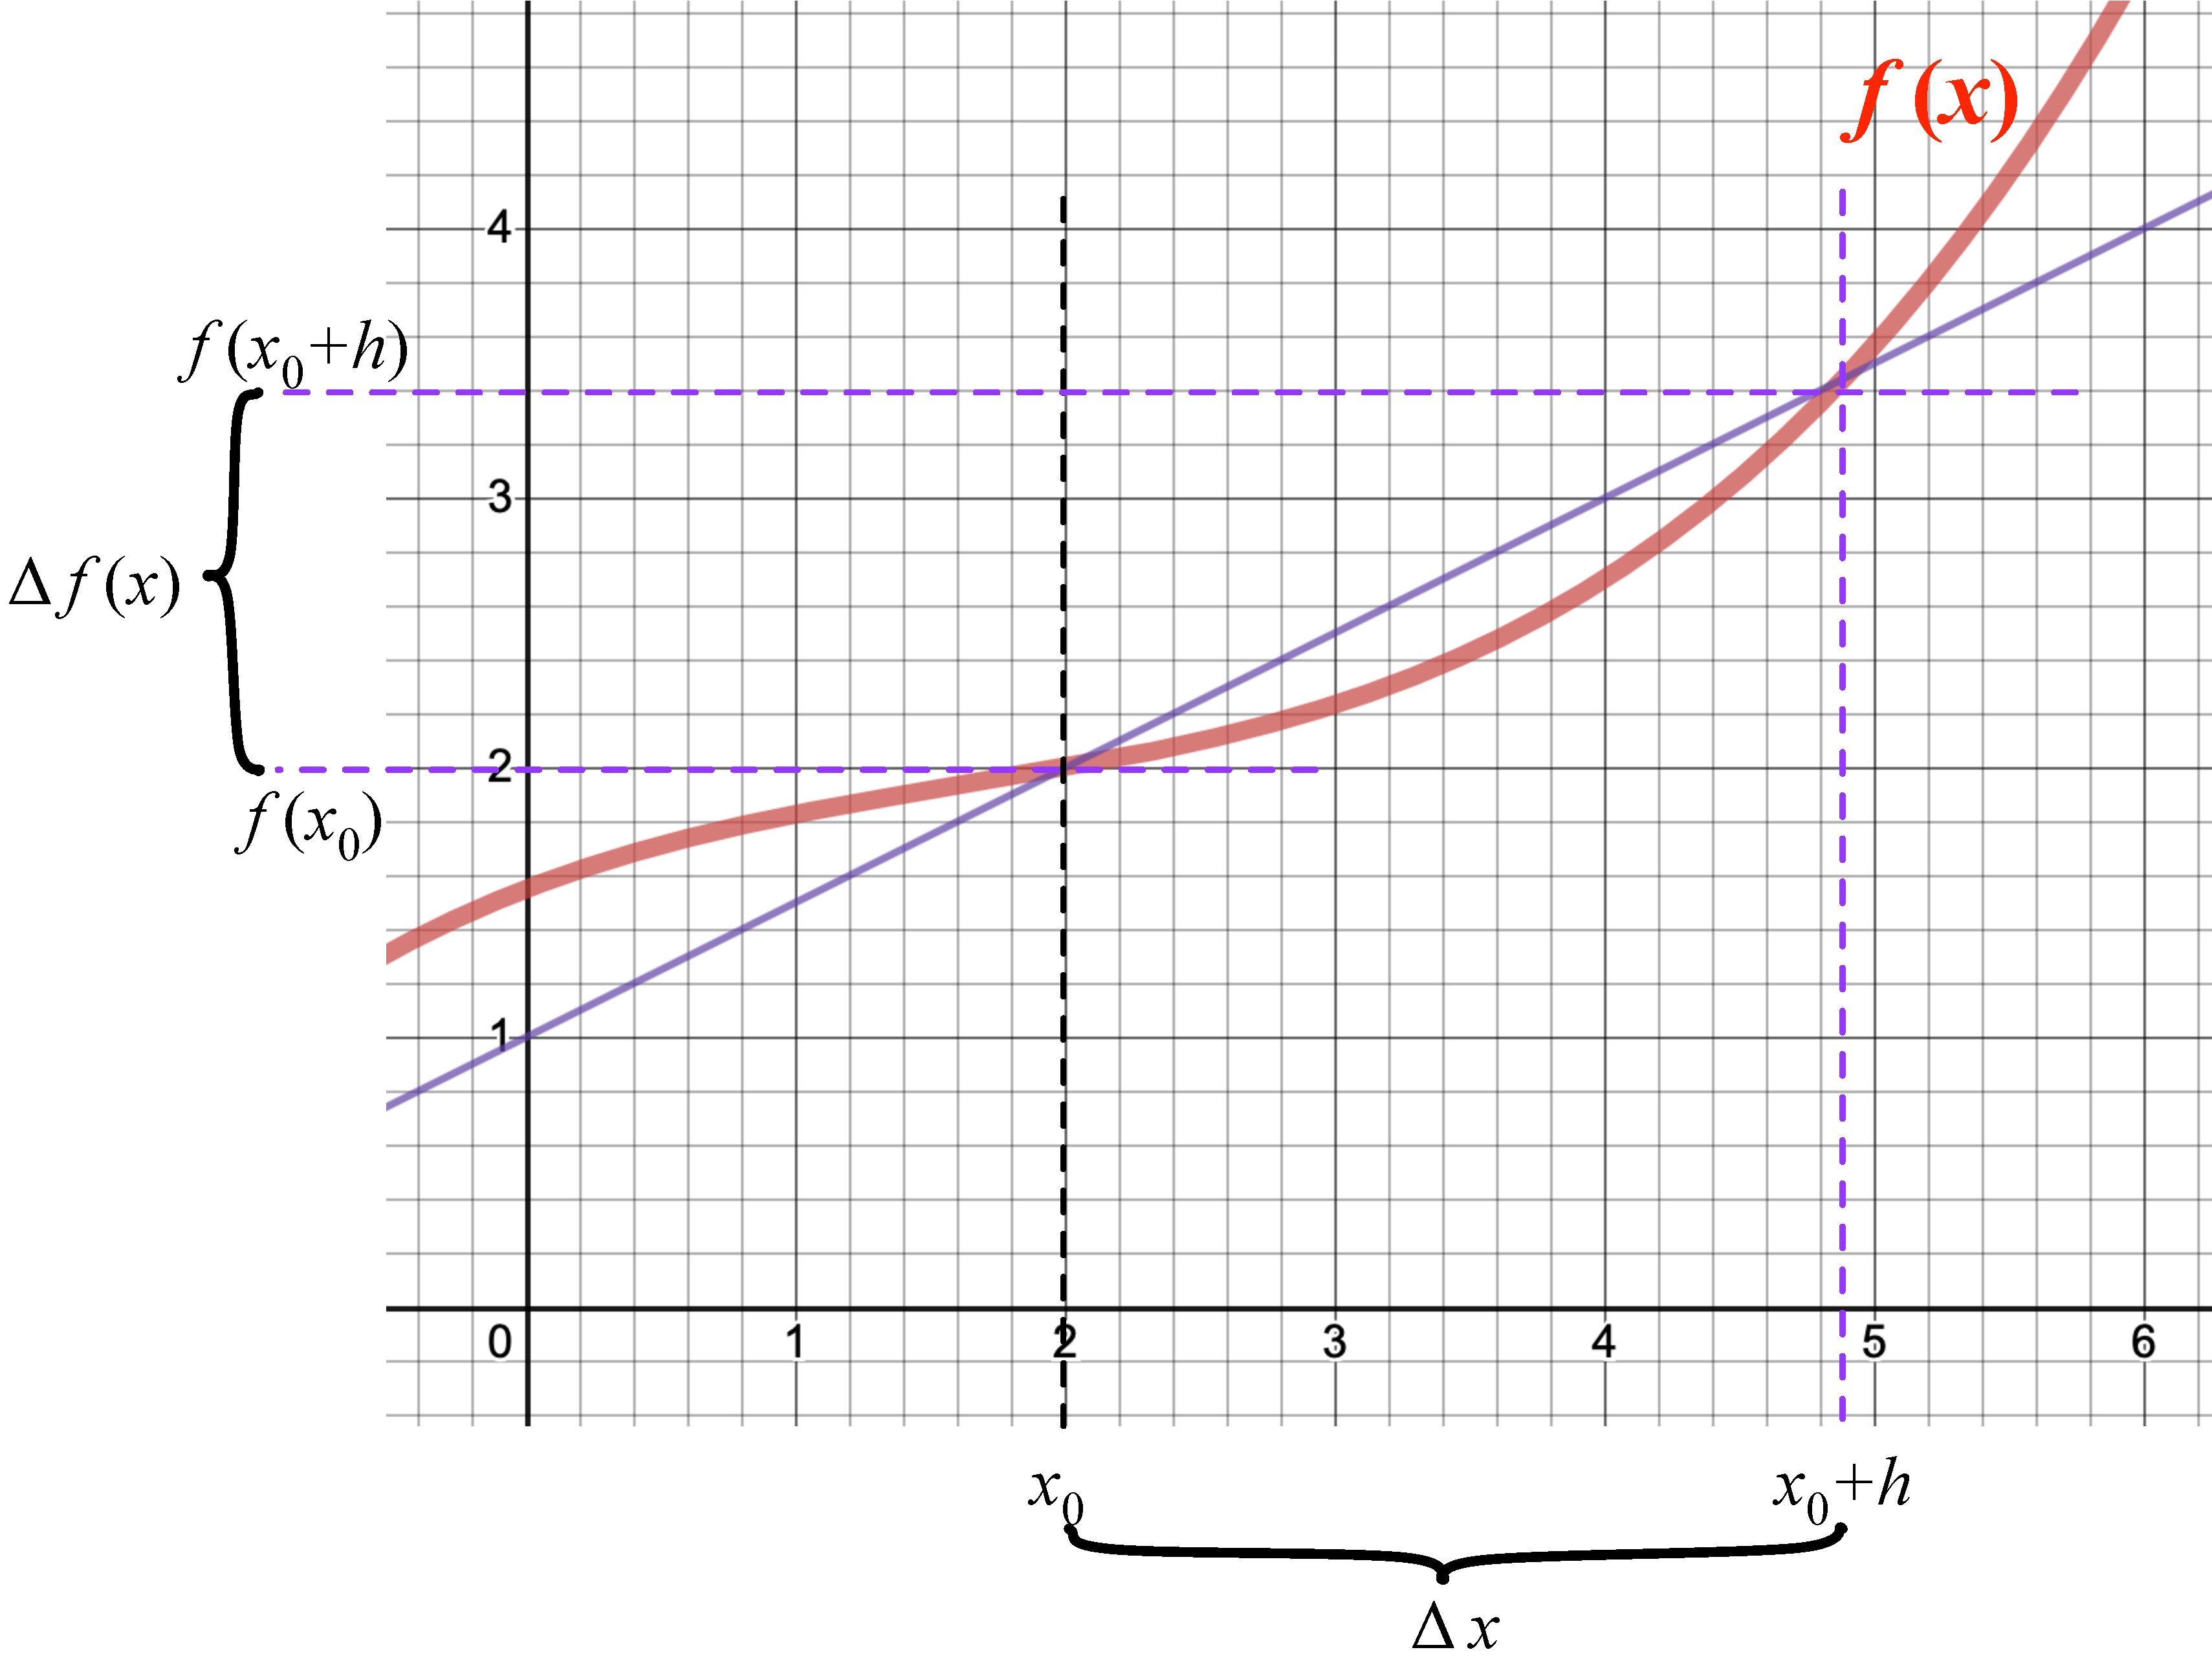
\includegraphics[width=8cm]{pic/SecantSlope.pdf}
\anngraphics{8cm}{pic/SecantSlope.png}{A secant line connects two points on
a graph within a coordinate plane.}
\end{center}
\caption{A secant}
\label{figonesecant}
\end{figure}

\begin{figure}
\begin{center}
%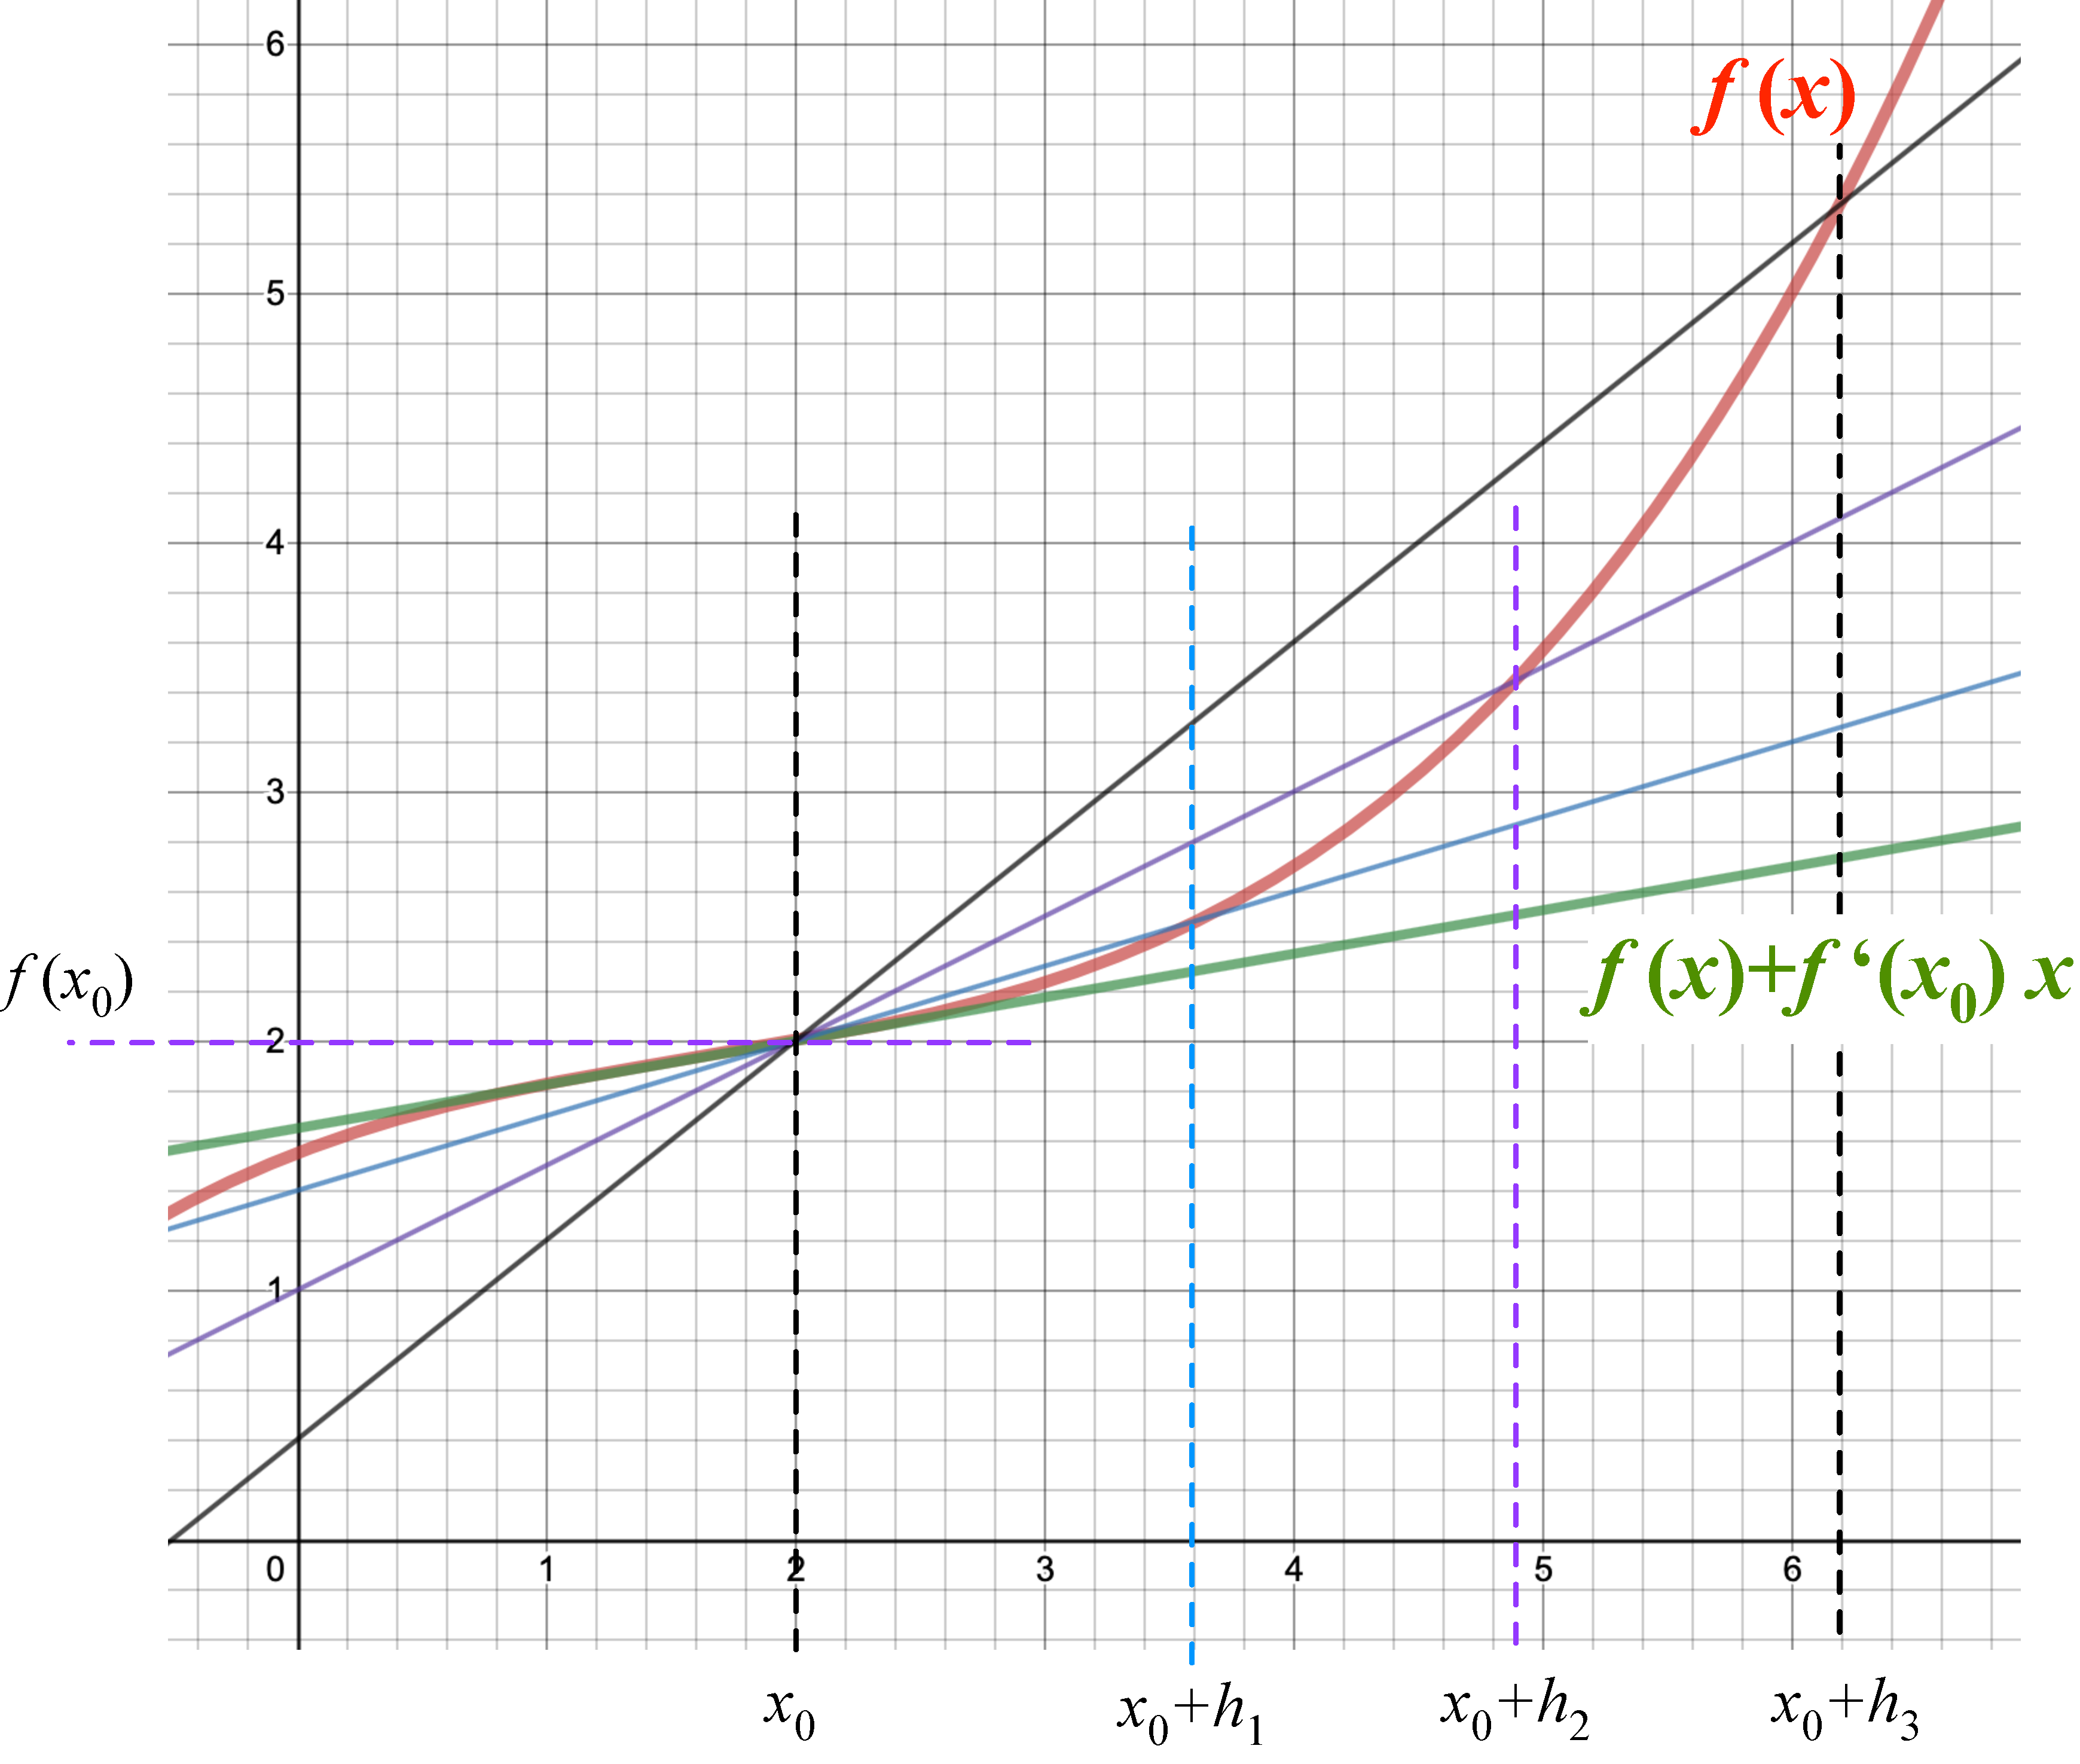
\includegraphics[width=8cm]{pic/SecantSlopes.pdf}
\anngraphics{8cm}{pic/SecantSlopes.png}{Multiple secant lines are shown on a
coordinate plane and contrasted with the tangent line, which is only
dependent upon one point on the graph instead of two.}
\end{center}
\caption{Multiple secants and the tangent}
\label{figsecantslopes}
\end{figure}

We can deal with this variability by not considering the absolute change
$f(x_0+1)-f(x_0)$ by one unit, but by
considering a variable step width (which we denote by $h$ or by
$\Delta x$, $\Delta$ being used here to indicate a difference), and to
consider the change relative to the step width. That is, we consider the
fraction
\begin{equation}
\frac{f(x_0+h)-f(x_0)}{(x_0+h)-x_0}=\frac{f(x_0+h)-f(x_0)}{h}
\label{diffquot}
\end{equation}
This fraction is the slope of the line between the points $(x_0,f(x_0))$ and
$(x_0+h,f(x_0+h))$, Figure~\ref{figonesecant}. Such a line is called a \defini{secant}, as it intersects the graph
twice. The ratio in equation~(\ref{diffquot}) gives the slope of this secant, and
is called the \defini{difference quotient}.
Since the numerator is the change of
function values, sometimes this quotient is also written as $\displaystyle
\frac{\Delta f(x)}{\Delta x}= \frac{\Delta y}{\Delta x}$.

But we can choose different values of $h$ (Figure~\ref{figsecantslopes}),
and (unless the function is a line) this will yield different secants with
different slopes, depending on the value of $h$.

To remove this ambiguity we now make $h$ small. That is, we consider
the difference quotient as a function of $h$ and study the limit
\[
\lim_{h\to 0}\frac{f(x_0+h_n)-f(x_0)}{h_n}
\]
This limit (if it exists) is the slope of the tangent line to the graph of
$f$ at $x_0$.
\smallskip

This approach immediately raises two questions:

\paragraph{Will this limit always exist?} No. It is possible that the limit
does not exist, for example if the function is not continuous at $x_0$. Also
the limit might not exist.
For example, if the graph
has a ``corner'' at $x_0$ (as the graph for $\sz{x}$ has at $x_0=0$), the
limit for a sequence of positive $h_n$ will differ from the limit of a
sequence of negative $h_n$. The formal definition thus needs to require this
limit to exist:

\begin{defn}
Let $f\colon\R\to\R$ be a function that is continuous at $x_0$. If the limit
\[
L=\lim_{h\to 0}\frac{f(x_0+h_n)-f(x_0)}{h_n}
\]
exists, then
$f$ is called \defini{differentiable} at $x_0$. The value $L$ (which is the
slope of the tangent to the graph of $f$ at $x_0$) is called the
\defini{derivative of $f$ at $x_0$} and denoted by $f'(x_0)$.
\end{defn}
Note that in particular that a function that is not continuous at $x_0\in\R$
is not differentiable at $x_0$. But there are continuous functions that are
not differentiable. Figure~\ref{fiUndifferentiable} shows some typical situations:
\begin{itemize}
\item The function tends to infinity (so might not even be continuous).
\item The slope becomes vertical at a point.
\item The graph of the function has a ``kink'', so there will not be a
unique tangent.
\end{itemize}
\begin{figure}[t]
\begin{center}
%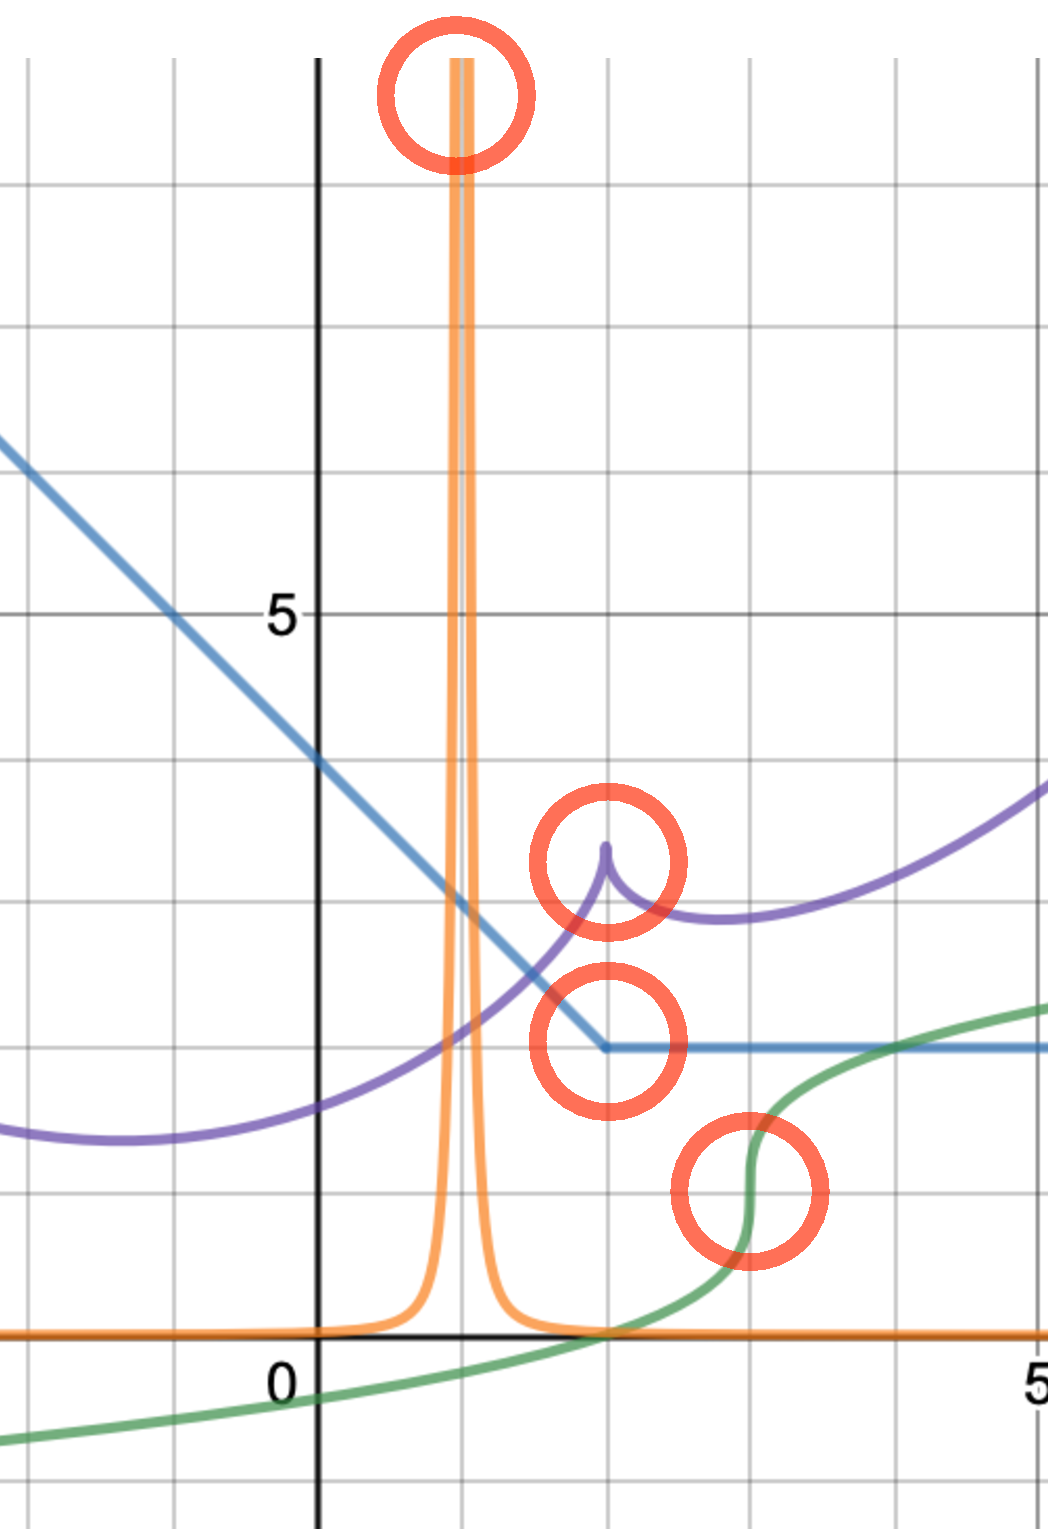
\includegraphics[width=5cm]{pic/Undifferentiable.pdf}
\anngraphics{5cm}{pic/Undifferentiable.png}{Corners, cusps, vertical asymptotes, and
purely vertical lines are depicted on a coordinate plane and labelled as
being undifferentiable.}
\end{center}
\caption{Not differentiable}
\label{fiUndifferentiable}
\end{figure}

\paragraph{How can we test for being differentiable,
and calculate the value of the derivative?}
Testing differentiability can be technical and is not a focus in this
course. We will see how this works in a few easy examples, but then
introduce easier rules for finding derivatives.

\section{Basic Derivatives, Polynomials}
\label{secderpol}

Let us consider a few easy cases. First, consider a constant function
$f(x)=c$. In this case $f(x_0)=c=f(x)$ for every $x$ and thus
\[
\frac{f(x_0+h_n)-f(x_0)}{h_n} =\frac{c-c}{h_n}=0
\]
and thus the limit exists, and is always equal
\[
\lim_{n\to\infty} \frac{f(x_0+h_n)-f(x_0)}{h_n}=0
\]
Therefore: A constant function is differentiable at every $x_0$, and has
derivative $f'(x_0)=0$.

Next consider the function $f(x)=x$. Then
\[
\frac{f(x_0+h_n)-f(x_0)}{h_n} =\frac{(x_0+h_n)-x_0}{h_n}=\frac{h_n}{h_n}=1.
\]
Again, the limit exists, and is always equal and we have that
$f'(x_0)=1$.

For the next cases, we will need the limit laws from
Lemma~\ref{limitlaws}: Consider the function $f(x)=x^a$ for an integer
$a>1$. Then (by the binomial theorem~\mynote{recall Pascal's triangle}) we
have that
\[
f(x_0+h_n)=(x_0+h_n)^a=\sum_{i=0}^a {a\choose i} x_0^{a-i} h_n^i
=x_0^a+\sum_{i=1}^{a} {a\choose i} x_0^{a-i} h_n^i
\]
and thus
\begin{eqnarray*}
\frac{f(x_0+h_n)-f(x_0)}{h_n}&=&\frac{(x_0+h_n)^a-x_0^a}{h_n}
=\frac{x_0^a+\sum_{i=1}^{a} {a\choose i} x_0^{a-i} h_n^i-x_0^a}{h_n}\\
&=&\frac{\sum_{i=1}^{a} {a\choose i} x_0^{a-i} h_n^{i}}{h_n}
=\sum_{i=1}^{a} {a\choose i} \frac{x_0^{a-i} h_n^{i}}{h_n}
=\sum_{i=1}^{a} {a\choose i} x_0^{a-i} h_n^{i-1}\\
&=&a x_0^{a-1}+\sum_{i=2}^a{a\choose i} x_0^{a-i} h_n^{i-1}.
\end{eqnarray*}
But every summand in the sum on the right hand side has a factor $h_n$ and,
since $\lim_{n\to\infty h_n}=0$ we have
$\lim_{n\to\infty}\sum_{i=2}^a{a\choose i} x_0^{a-i} h_n^{i-1}=0$ and thus
\[
\lim_{n\to\infty}\frac{(x_0+h_n)^a-x_0^a}{h_n}=a x_0^{a-1}.
\]
Once more, the limit exists and is independent of the choice of sequence
$h_n$. Thus the function $f(x)=x^a$ is differentiable at every $x_0$ and has
the derivative $f'(x_0)=a x^{a-1}$. This result subsumes (for $a=0$ and
$a=1$ the previous two, and one can show that it even holds if $a$ is an
arbitrary real number.
\smallskip

A similar application of the limit laws gives us that, if $f$ and $g$ are
differentiable at $x_0$, so is  $(f+g)(x)$ with derivative
$f'(x_0)+g'(x_0)$, as is $(cf)(x)$ (for a constant $c\in\R$) with derivative
$cf'(x_0)$.
\smallskip

Combining all of this, we have that a polynomial $f(x)=\sum_{i=0}^n a_ix^i$
is differentiable at every $x_0$ and has the derivative\mynote{and this is
all you need to remember from this section!}
\[
f'(x_0)=\sum_{i=1}^n a_i\cdot i\cdot x_0^{i-1}
\]

\section{The Derivative as a Function}

We have so far, for a given function $f$ defined a derivative at a point
$x_0$, as the slope of the tangent line to the graph of the function at
point $(x_0,f(x_0))$ and denoted it as $f'(x_0)$. Assuming the function $f$
is differentiable at every
$x_0\in\R$, we can calculate these derivative values $f'(x_0)$ for every
$x_0$ and consider $f'$ as a function itself (that assigns to $x_0$ the
value $f'(x_0)$). This function is called the derivative (function) of $f$.
Besides the name $f'$, it also is denoted by
$\displaystyle\frac{\mbox{d}f}{\mbox{d}x}$ or
$\displaystyle\frac{\mbox{d}}{\mbox{d}x} f$, where the
$\frac{\mbox{d}}{\mbox{d}x}$ is to be considered as a particular symbol
(alluding to the difference quotient), not
as an actual fraction. In Physics, also the notation $\dot f$ is sometimes
used.

This derivative function assigns to every point $x$ the slope of the tangent
to the graph of $f$ at the point $(x,f(x))$.
We already know how to determine a formula for this derivative function for
polynomials:
\begin{bsp}
Let $f(x)=x^{5}+x^{4}-20x^{3}-20x^{2}+64x+64$.
Figure~\ref{figmultitangent} shows tangents (green) to the graph (red) of $f$
at some points. If we determine the slope of these tangents at all points
$(x,f(x))$, we get the graph (blue) of the derivative $f'(x)$.

By the result of the previous section, we actually can calculate a formula
for this derivative as $f'(x)=5x^{4}+4x^{3}-60x^{2}-40x+64$. Using
this formula, we can calculate exact values of $f'(x)$ for arbitrary points $x$, as in the following table:
\[
\begin{array}{r|rrrrrrrrr}
x&-4&-3&-2&-1&0&1&2&3&4\\
\hline
f'(x)&288&-59&-48&45&64&-27&-144&-83&480
\end{array}
\]
Note that these values agree with the slopes of the tangents.
\end{bsp}
\begin{figure}[t]
\begin{center}
%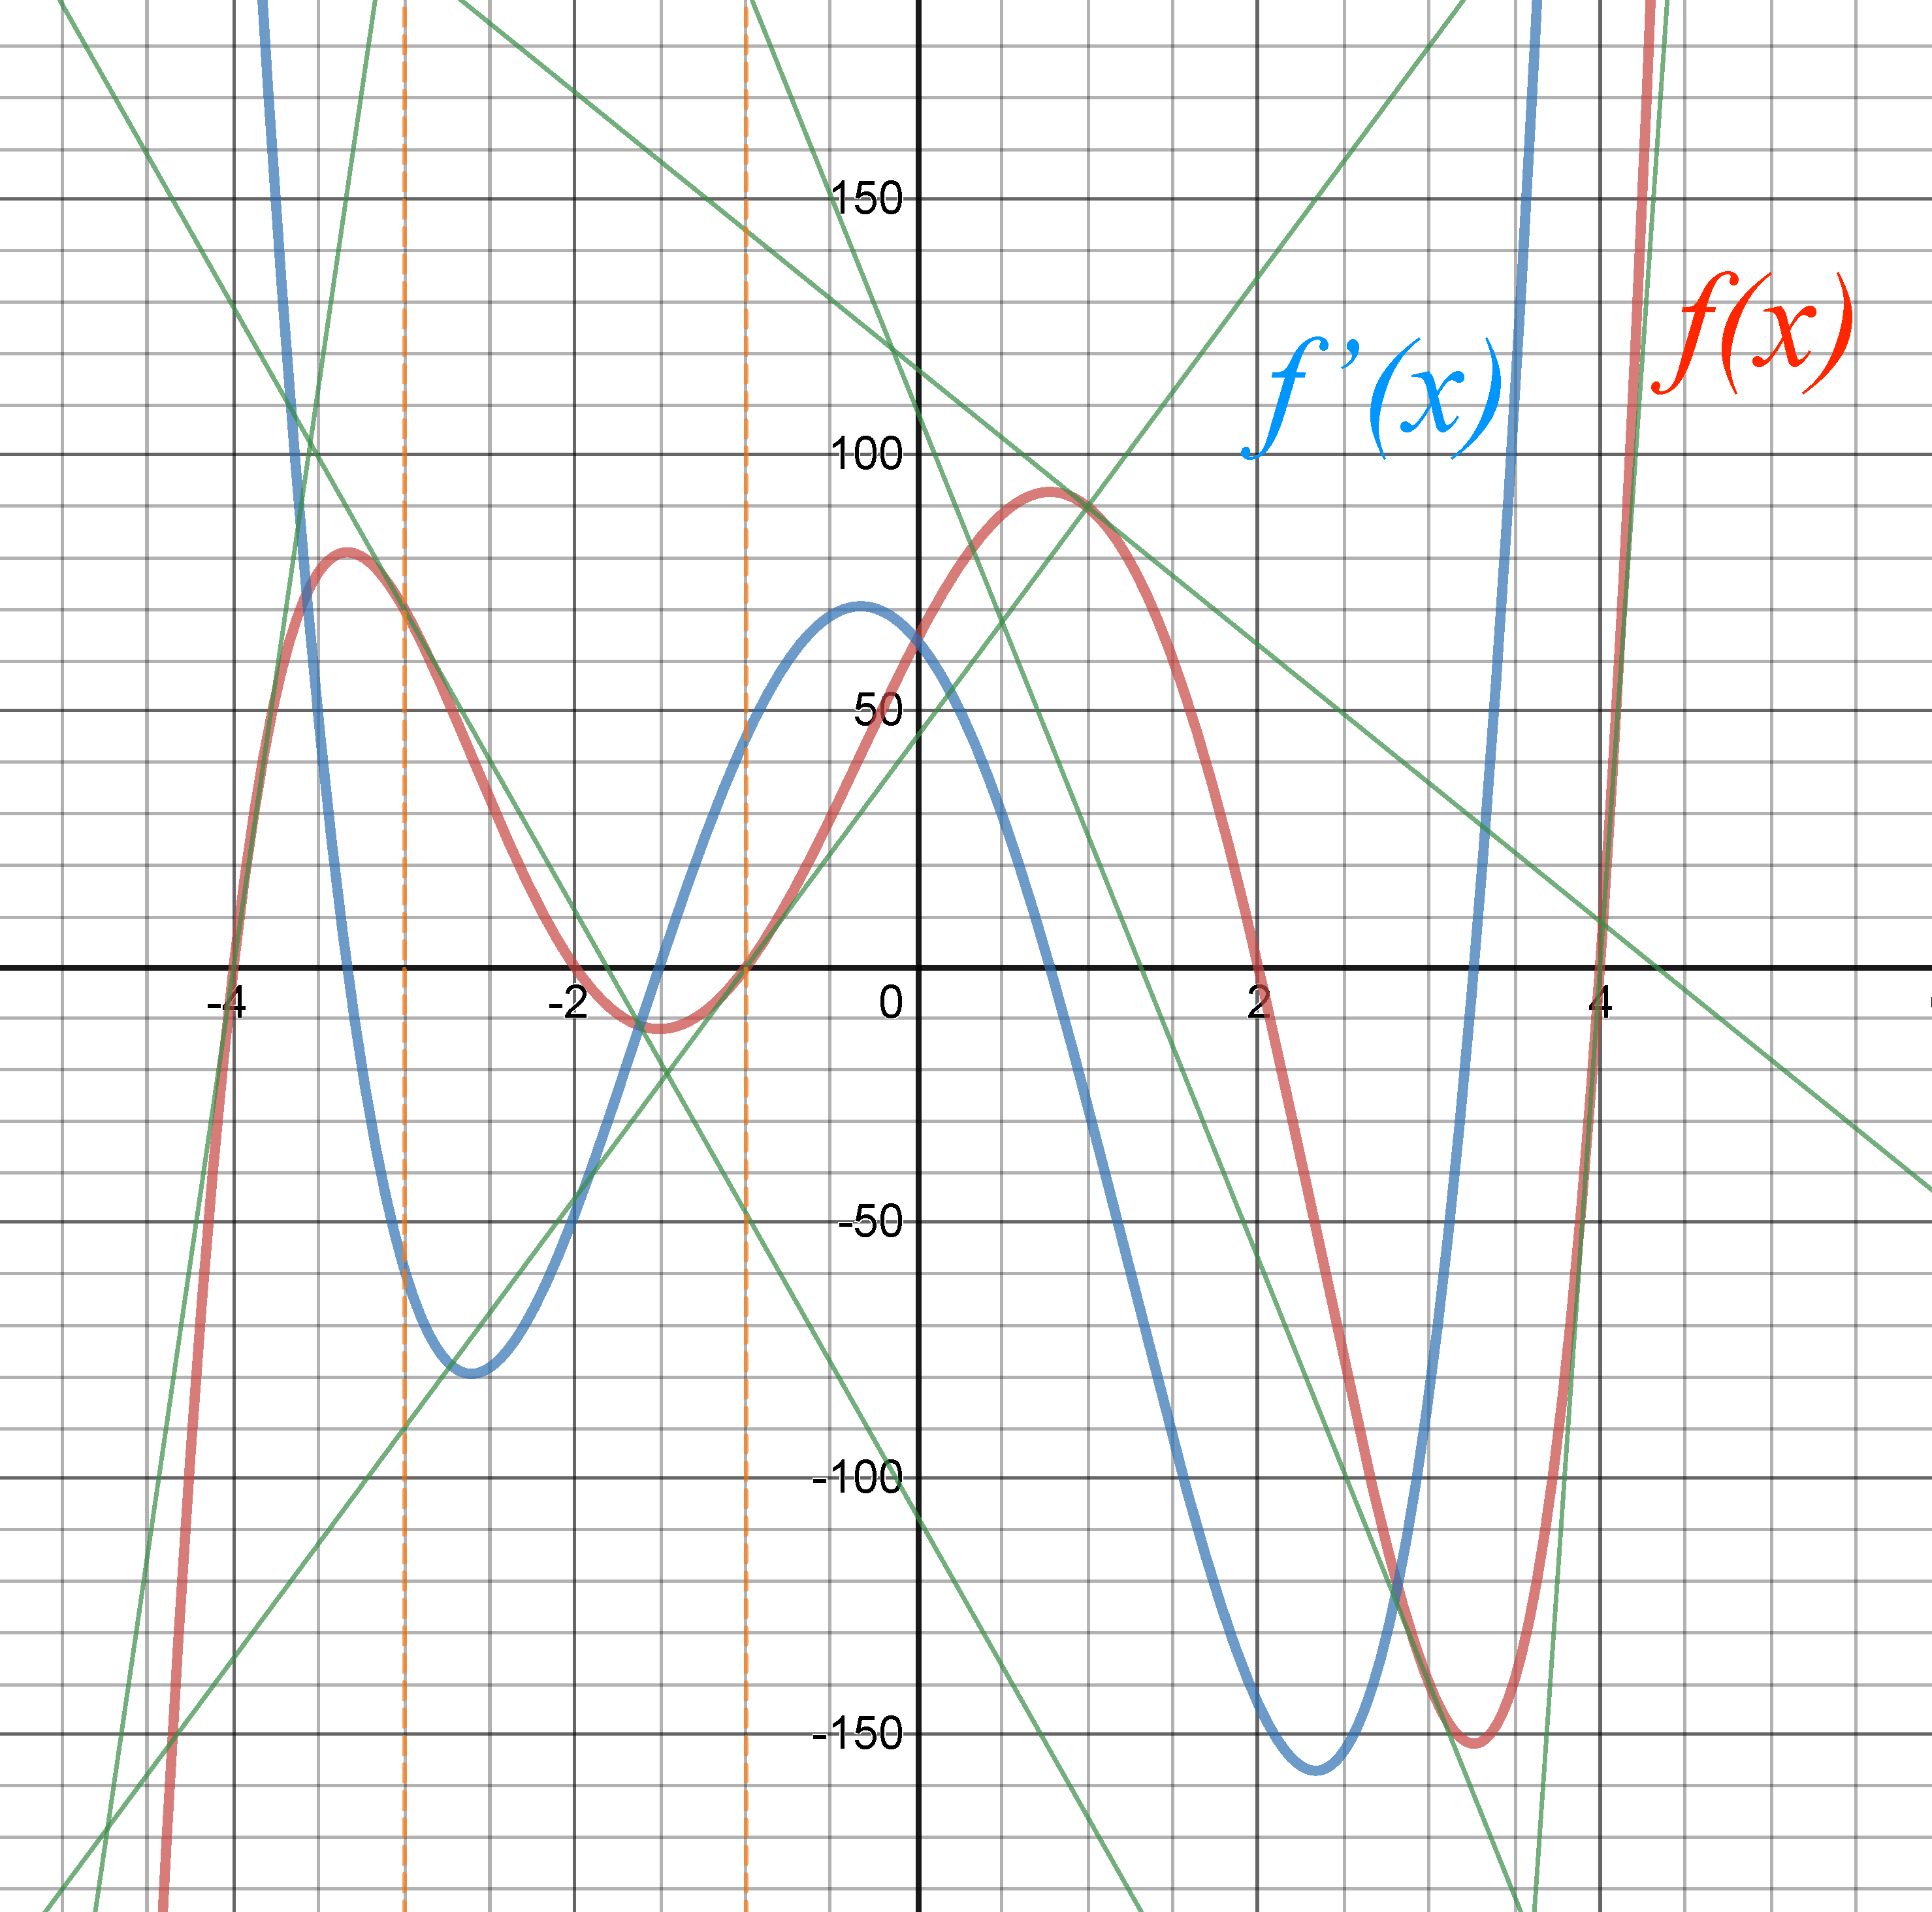
\includegraphics[width=8cm]{pic/MultiTangent.pdf}
\anngraphics{8cm}{pic/MultiTangent.png}{A graph $f(x)$ is plotted on a
coordinate plane. Tangent lines are shown on the graph of $f(x)$; the slopes
of these tangent lines become the y-values of $f'(x)$, the graph of the
derivative.}
\end{center}
\caption{Multiple tangents and the derivative}
\label{figmultitangent}
\end{figure}

\begin{note}
The notation $\displaystyle\frac{\mbox{d}f}{\mbox{d}x}$ serves another
purpose, namely indicating with respect to {\em which} variable we take the
derivative. If we look at multiple functions (or functions with a
parameter), a function expression might contain other symbols, though only
one will be considered the variable with respect to which we take the
derivative. In the case of $\displaystyle\frac{\mbox{d}f}{\mbox{d}x}$ this
variable is $x$, though one also might write
$\displaystyle\frac{\mbox{d}f}{\mbox{d}a}$ to indicate that the relevant
variable is called $a$.

Ultimately, of course such functions with be considered as being of multiple
variables, and the derivative with respect to one variable means we are
considering only a ``slice'' of the function. More about this will come in
multivariable calculus.

Here we just should note that e.g.
$\displaystyle\frac{\mbox{d}f}{\mbox{d}a}=x^2$ for $f(x)=a\cdot x^2$,
(considering $a$ as the variable and $x$ as constant), while
$\displaystyle\frac{\mbox{d}f}{\mbox{d}x}=a$ and
$\displaystyle\frac{\mbox{d}f}{\mbox{d}b}=0$.
\end{note}

\section{Derivatives of Elementary Functions}
\label{derelem}

A function is called \defini{elementary}\mynote{my dear Watson}, if it
cannot be composed from other functions. These are typically functions
that are useful in particular applications and that have their own key on the calculator, such as $\exp(x)$ or $\sin(x)$.

By careful inspection of the graphs of some of these functions it is possible
to identify expressions for their derivatives, we give one example of this
below. (The ultimate justification
for some of these formulas will for us come through Taylor
series~\ref{sectaylors}.)

We note these derivative formulas in the following table:

\[
\begin{array}{c|c}
\mbox{Function $f(x)$}&\mbox{Derivative $f'(x)$}\\
\hline
\sin(x)&\cos(x)\\
\cos(x)&-\sin(x)\\
\exp(x)=e^x&\exp(x)\\
\log(x)&1/x\\
\arcsin(x)&\frac{1}{\sqrt{1-x^2}}\\
\arccos(x)&\frac{-1}{\sqrt{1-x^2}}\\
\arctan(x)&\frac{-1}{1+x^2}\\
\mbox{bla}(x)&\frac{e^x-1}{x}\\
\end{array}
\]
This table also gives an indication what is special about the basis $e$ in
the exponential function $\exp(x)=e^x$, as for this basis the function equals
its own derivative.

\begin{note}
The reader will note a function $\mbox{bla}(x)$, that she did not
encounter before. It is a made-up function that is introduced solely to
provide example problems for homework and exams that cannot be solved with standard
computational tools.
\end{note}

\begin{bsp}
% TN, edited by AH
We have seen in Section~\ref{secderpol} a proof of the formula for
differentiating polynomials. Here we give a similar argument for why
$\displaystyle\frac{\mbox{d}\sin(x)}{\mbox{d}x}=\cos(x)$:

To establish this we need to show that
\[\lim_{h \to 0}\frac{\sin(x+h)-\sin(x)}{h} = \cos(x).\]
Recall from trigonometry that $\sin(x+h) = \sin(x)\cos(h) + \cos(x)\sin(h)$. Then some algebra and application of limit properties yields
\begin{equation*}
\begin{split}
\lim_{h \to 0}\frac{\sin(x+h)-\sin(x)}{h} &= \lim_{h \to 0} \frac{\sin(x)\cos(h) + \cos(x)\sin(h) - \sin(x)}{h} \\
&= \lim_{h \to 0} \bigg(\frac{\sin(x)\big(\cos(h)-1\big)}{h} + \frac{\cos(x)\sin(h)}{h} \bigg) \\
&= \sin(x) \lim_{h \to 0}\bigg(\frac{\cos(h)-1}{h}\bigg) + \cos(x)\bigg(\lim_{h \to 0}\frac{\sin(h)}{h}\bigg).\\
\end{split}
\end{equation*}

It remains to evaluate the limits. Toward that end let us analyze the graphs
of the two summands. Figure~\ref{tnex1figs}, shows on the left the graph of
$\frac{\cos(h)-1}{h}$ around $h=0$, while the right side shows the graph of
$\frac{\sin(h)}{h}$ around $h=0$.

\begin{figure}
\begin{center}
%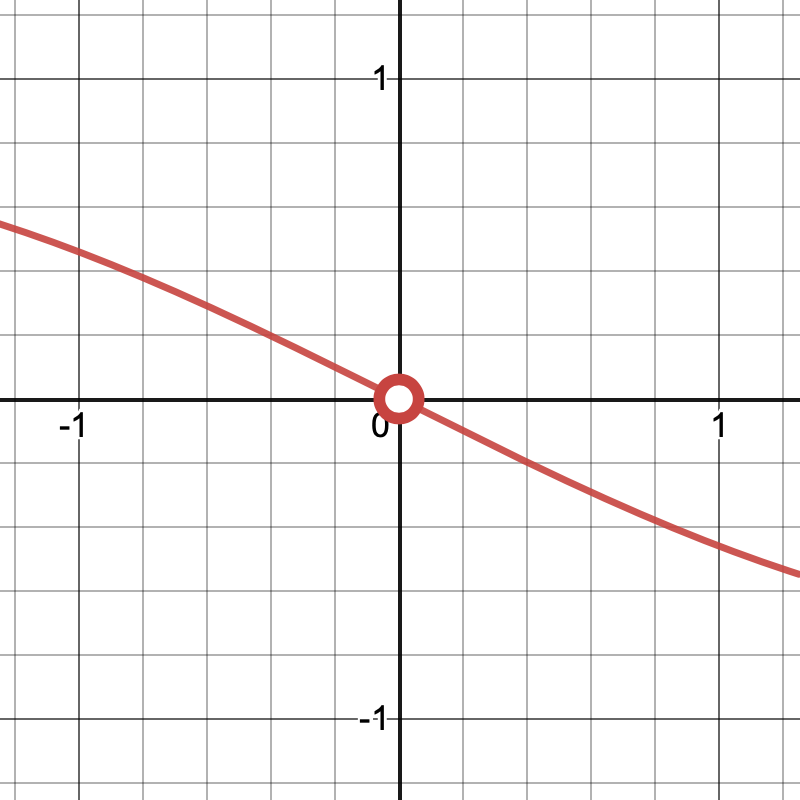
\includegraphics[width=4cm]{pic/tnex1pic1.png}
\anngraphics{4cm}{pic/tnex1pic1.png}{Graph for (cos(h)-1)/h, showing that
the undefined value at x=0 can be added in a way that makes the function
continuous.}
\qquad
%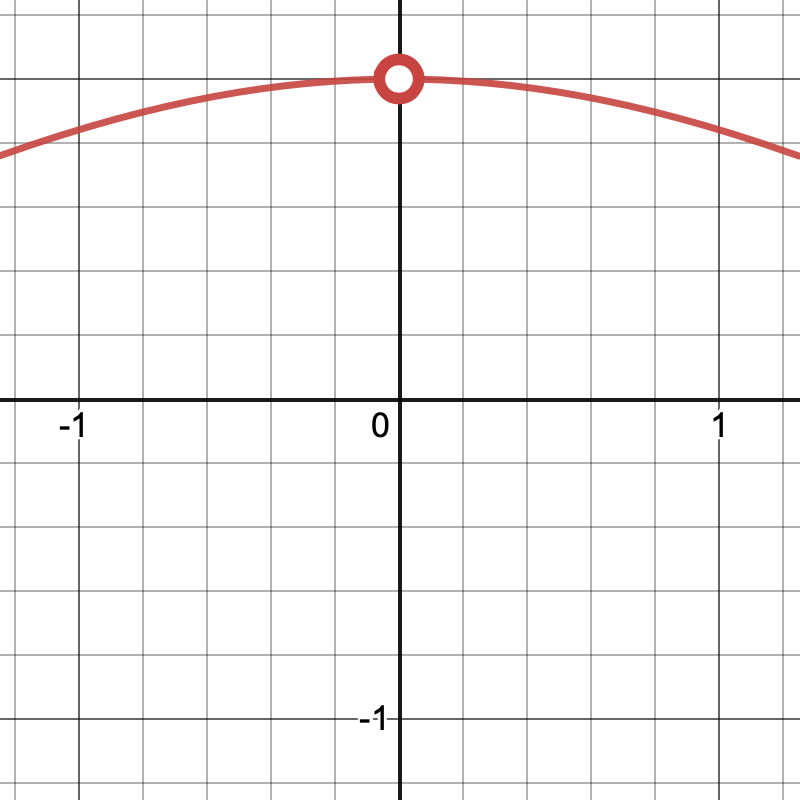
\includegraphics[width=4cm]{pic/tnex1pic2.png}
\anngraphics{4cm}{pic/tnex1pic2.png}{Graph for sin(h)/h, showing that
the undefined value at x=0 can be added in a way that makes the function
continuous.}
\end{center}
\caption{Graphs of $\frac{\cos(h)-1}{h}$ and $\frac{\sin(h)}{h}$, for
$h\neq0$}
\label{tnex1figs}
\end{figure}


From these graphs we see that
\[
\lim_{h \to 0}\frac{\cos(h)-1}{h} = 0, \quad\mbox{and}\quad \lim_{h \to 0}\frac{\sin(h)}{h} = 1
\]
Putting it all together we find
\[\lim_{h \to 0}\frac{\sin(x+h)-\sin(x)}{h} = \sin(x) \cdot 0 + \cos(x) \cdot 1 = \cos(x)\]
which is what we wanted to show.

There is (of course) a formal, non-graphical, way to derive these limits which
requires some as well as a theorem from advanced calculus, called the
``squeeze theorem" (or ``sandwich theorem"), which is beyond the scope of
this text. Alternatively, we will see an argument involving Taylor series
later in the text.
\end{bsp}

\section{Differentiation Rules}

When we studied functions, we looked at how we can build new functions from
simpler ones. These constructions also allow us to write down formulas for the
derivatives, as we will study in this section. We will aim to give a
justification for each of these formulas, though will not always give a
formal proof.

Let us start with some basic cases. (Some of these will end up later just
being special cases of a more general rule, so you won't have to memorize
all of this, but it is to help justifying the more general cases.)

We start with the basic transformations to a function's graph, as in
section~\ref{secfunari}. Let us look at the graph of a function under
transformations, and see how this affects the slope of a secant. (Since the
derivative is the slope of a tangent as limit of the secant slope, it will
be transformed in the same way.)

In the examples in Figure~\ref{figderbasic}, we always transform an original function $f$
(red) and its secant (orange) (from $x_0=0$ to $x_0+h=8$)
to a new function $p$ (blue, with
corresponding green secant). Recall that the slope of the secant is given as
\[
\frac{\Delta f}{\Delta x}=\frac{f(x_0+h)-f(x_0)}{x_0+h-x_0}
=\frac{f(x_0+h)-f(x_0)}{h},
\]
and that we thus only need to see how $\Delta f$ and/or $\Delta x$
transform. Note that vertical shift can be considered as a special case of
addition, and that the rules for addition and for vertical scaling
agree with what we've seen before in Section~\ref{secderpol} for
polynomials.

\begin{figure}
\begin{tabular}{cccc}
\begin{minipage}[b]{4cm}
%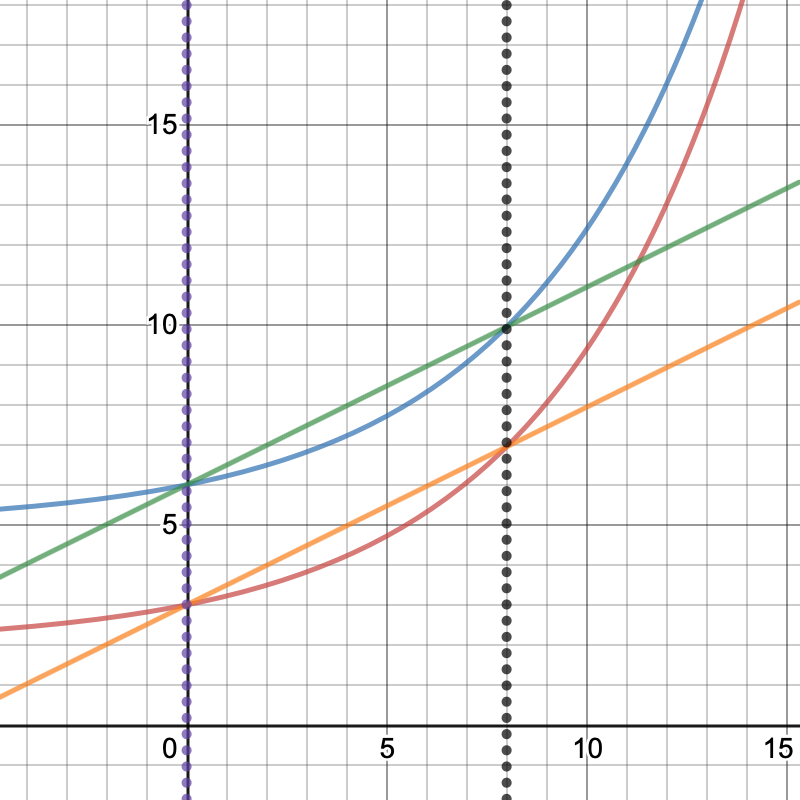
\includegraphics[width=4cm]{pic/picder1.png}%
\anngraphics{4cm}{pic/picder1.png}{A vertical shift in a graph, with its
corresponding secant lines, illustrated on a coordinate plane.}
\end{minipage}&
\begin{minipage}[b]{3cm}
\textbf{Vertical Shift:}\\
$p(x)=f(x)+3$.
Then $\Delta p=\Delta f$ and $\Delta x$ stays the same:
\[
\frac{\Delta p}{\Delta x}=\frac{\Delta f}{\Delta x}
\]
\vfill\
\end{minipage}&&\begin{minipage}[b]{3cm}
$p'(x)=f'(x)$.
\vspace{2cm}
\vfill\
\end{minipage}\\
\begin{minipage}[b]{4cm}
%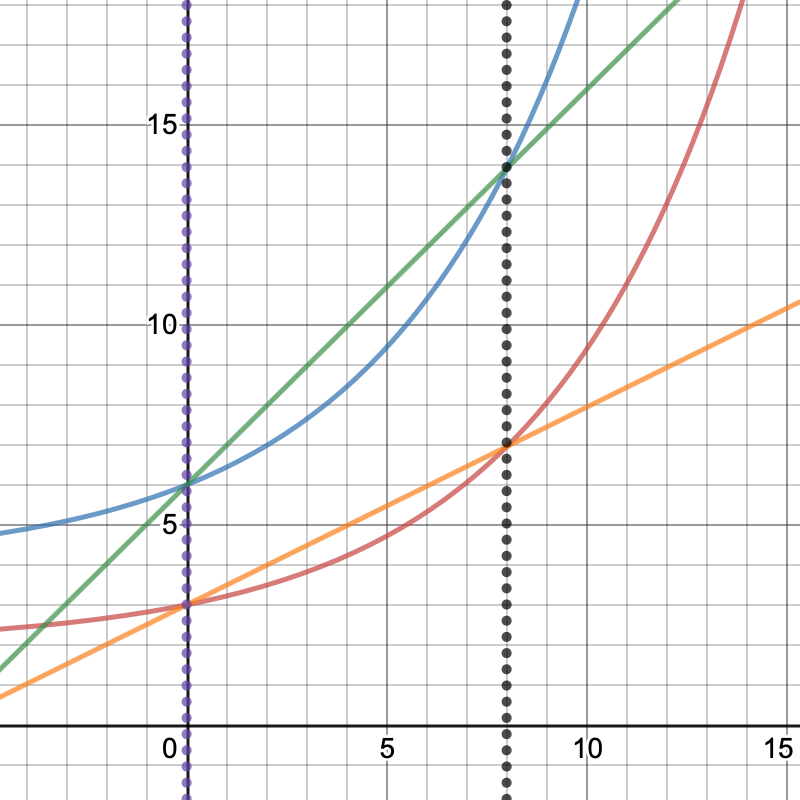
\includegraphics[width=4cm]{pic/picder2.png}%
\anngraphics{4cm}{pic/picder2.png}{A vertical scaling of a graph, with its
corresponding secant lines, illustrated on a coordinate plane.}
\end{minipage}&
\begin{minipage}[b]{3cm}
\textbf{Vertical Scaling:}\\
$p(x)=2\cdot f(x)$.
Then $\Delta p=\Delta f$ and $\Delta x$ stays the same.
\[
\frac{\Delta p}{\Delta x}=2\frac{\Delta f}{\Delta x}
\]
\vfill\
\end{minipage}&&\begin{minipage}[b]{3cm}
$p'(x)=2\cdot f'(x)$.
\vspace{2cm}
\vfill\
\end{minipage}\\
\begin{minipage}[b]{4cm}
%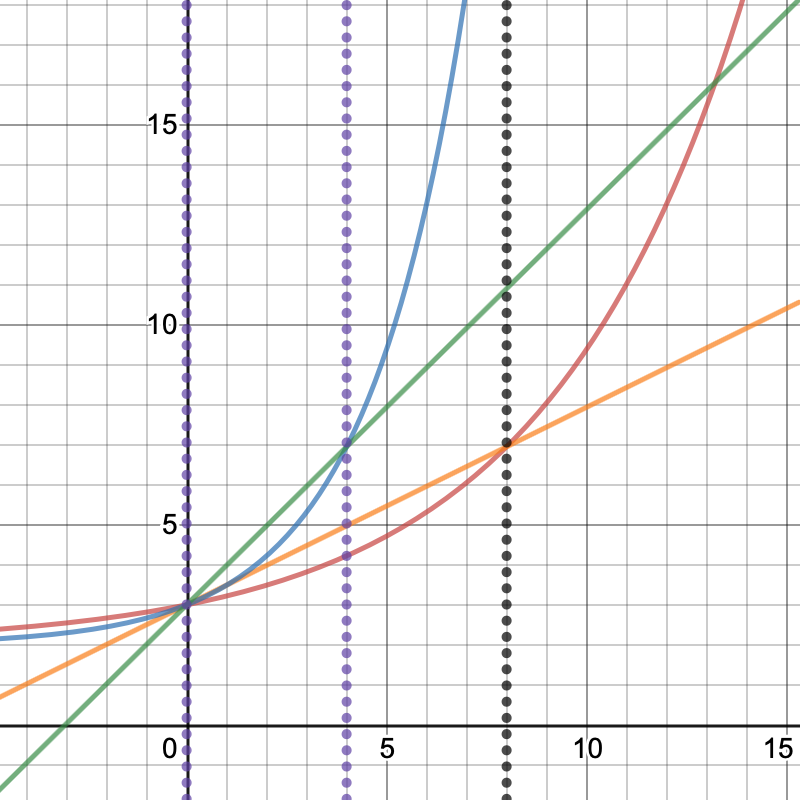
\includegraphics[width=4cm]{pic/picder3.png}
\anngraphics{4cm}{pic/picder3.png}{A horizontal scaling of a graph, with its
corresponding secant lines, illustrated on a coordinate plane.}
\end{minipage}&
\begin{minipage}[b]{3cm}
\textbf{Horizontal Scaling:}\\
$p(x)=f(2\cdot x)$.
Then $\Delta p=\Delta f$, but $\Delta x$ shrinks by a factor $2$.
\[
\frac{\Delta p}{\Delta x}=\frac{\Delta f}{\Delta x/2}=2\frac{\Delta f}{\Delta x}
\]
\vfill\
\end{minipage}&&\begin{minipage}[b]{3cm}
$p'(x)=2\cdot f'(x)$.
\vspace{2cm}
\vfill\
\end{minipage}\\
\begin{minipage}[b]{4cm}
%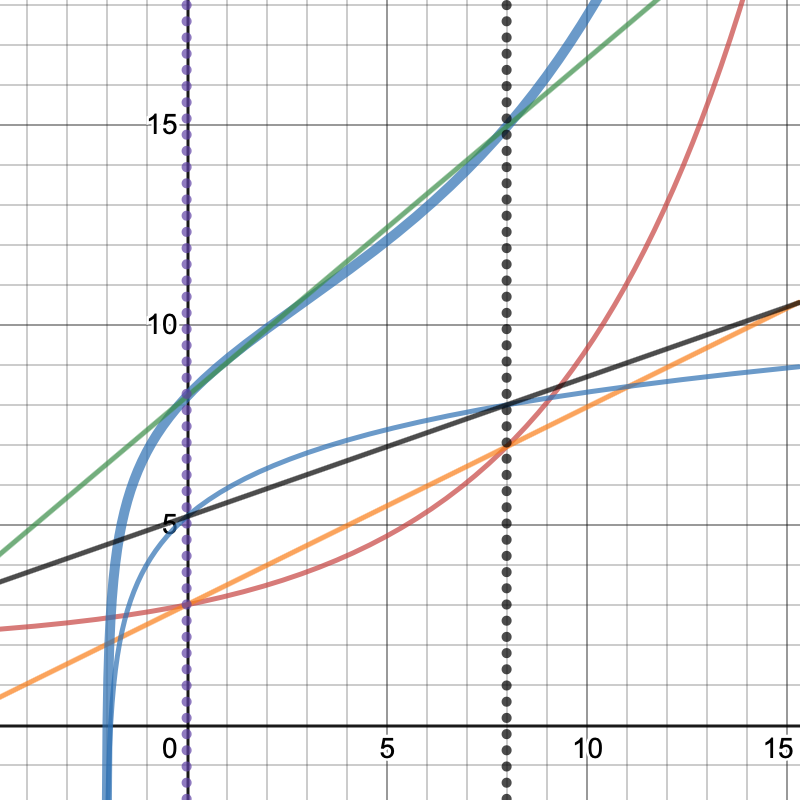
\includegraphics[width=4cm]{pic/picder4.png}%
\anngraphics{4cm}{pic/picder4.png}{Addition of two functions, with its
corresponding secant lines, is illustrated on a coordinate plane.}
\end{minipage}&
\begin{minipage}[b]{3cm}
\textbf{Addition:}\\
$p(x)=f(x)+g(x)$.
Then\\ $\Delta p=\Delta f+\Delta g$, and $\Delta x$ stays the same.
\[
\frac{\Delta p}{\Delta x}=\frac{\Delta f+\Delta g}{\Delta x}
\]
\vfill\
\end{minipage}&&\begin{minipage}[b]{3.5cm}
$p'(x)=f'(x)+g'(x)$.
\vspace{2cm}
\vfill\
\end{minipage}\\
\end{tabular}
\caption{Basic transformations of the derivative}
\label{figderbasic}
\end{figure}

\subsection{Product Rule}
Next, lets look at the case of a product of functions, that is we have that
$p(x)=f(x)\cdot g(x)$, and the function values change by $\Delta
f=f(x_0+h)-f(x_0)$,
respectively by $\Delta g=g(x_0+h)-g(x_0)$. Then (imagine $f$ and $g$ as
sides of a rectangle, whose area is $p$ and that changes as both sides
change length):
\begin{eqnarray*}
\Delta p&=&p(x_0+h)-p(x_0)=f(x_0+h)\cdot g(x_0+h)-f(x_0)g(x_0)\\
&=&\left(\Delta f+f(x_0)\right)\left(\Delta g+g(x_0)\right)-f(x_0)g(x_0)\\
&=&\Delta f\Delta g+\Delta f\cdot g(x_0)+f(x_0)\cdot \Delta g+f(x_0)g(x_0)-f(x_0)g(x_0)\\
&=&\Delta f\Delta g+\Delta f\cdot g(x_0)+f(x_0)\cdot \Delta g.\\
\end{eqnarray*}
If we now consider the value of the derivative as limit of the difference
quotient
\begin{eqnarray*}
p'(x_0)&=&\lim_{h\to 0}\frac{\Delta p}{\Delta x}
=\lim_{h\to 0}\frac{\Delta f\Delta g+\Delta f\cdot g(x_0)+f(x_0)\cdot
\Delta g}{\Delta x}\\
&=&\lim_{h\to 0}\frac{\Delta f\Delta g}{\Delta x}+\lim_{h\to 0}\frac{\Delta
f}{\Delta x}\cdot g(x_0)+f(x_0)\cdot\lim_{h\to 0}\frac{\Delta g}{\Delta x}\\
&=&f'(x_0)g(x_0)+f(x_0)g'(x_0)+\lim_{h\to 0}\frac{\Delta f\Delta g}{\Delta x}
\end{eqnarray*}
and observe that in the remaining limit the numerator $\Delta f\Delta g$
shrinks {\em twice as fast} (because of the double-$\Delta$) as the
denominator $\Delta x$. This limit is thus equal to zero and we get
(replacing $x_0$ by a general $x$) the \defini{product rule}
\[
p'(x)=f'(x)g(x)+f(x)g'(x),
\qquad \frac{\mbox{d}}{\mbox{d}x} (f\cdot
g)(x)=\frac{\mbox{d}f}{\mbox{d}x}(x)\cdot
g(x)+f(x)\cdot\left(\frac{\mbox{d}g}{\mbox{d}x}(x)\right)
\]

\subsection{Chain Rule (= Composition Rule)}
The case of composition of functions looks most complicated, as we have a
change depending on change.
Thus, let us first look at some easy examples of how such change
accumulates, namely the case of polynomials of degree one.

For example, imagine that a bicyclist ascends a mountain road,
at a rate of $3000$
foot/hr, starting at ground level (5000 ft). Measuring in units of hours and
1000 ft, her altitude after $x$ hours thus is $g(x)=5+3x$.
The temperature decreases by $2$ degree per thousand foot and is, at
altitude $a$, given as $f(a)=80-2a$. The temperature at time $x$ thus is
$p(x)=f(g(x))$. But how does the temperature change per time unit, i.e. what
is $p'(x)$? We can answer this in three different ways:

\begin{description}
\item[First,] in this example, we can evaluate $p(x)=f(g(x))=80-2(5+3x)=70-6x$ and
calculate the derivative $p'(x)=-6$. (That is per time unit, the temperature
decreases by 6 degrees.)

\item[Secondly,] we can observe that the composition consists of a horizontal
scaling by a factor of 3, and a left shift by $5$ units. The horizontal
scaling (as in the example in the previous section) will increase the slope
of secants and tangents by a factor of $3$. (The horizontal shift means that
the derivative values are shifted as the function is -- in this example this
will make no difference.) That is, we get the derivative of the function
$f$, which is $f'(a)=-2$, evaluated at $a=g(x)$, and multiplied by a factor
$3$, resulting in $p'(x)=-6$ as before.

\item[Thirdly,] we can work with the definition of the derivative as limit
of the difference quotient (and this
will work not just in this particular example). We have that
\[
\frac{\Delta p}{\Delta x}=\frac{\Delta p}{\Delta g}\cdot\frac{\Delta
g}{\Delta x}
\]
where we have set $\Delta g=g(x_0+h)=g(x_0)$ and
\[
\Delta p=p(x_0+h)-p(x_0)=f(g(x_0+h))-f(g(x_0)).
\]
Applying the limit rule for the product, we get
\begin{eqnarray*}
\lim_{h\to 0} \frac{\Delta p}{\Delta x}
&=&\lim_{h\to 0}\left(\frac{\Delta p}{\Delta g}\cdot\frac{\Delta g}{\Delta x}\right)
=\left(\lim_{h\to 0}\frac{\Delta p}{\Delta g}\right)\cdot\underbrace{\left(\lim_{h\to 0}\frac{\Delta
g}{\Delta x}\right)}_{=g'(x_0)}\\
&=&\lim_{h\to 0}\frac{f(g(x_0+h))-f(g(x_0))}{g(x_0+h)-g(x_0)}\cdot g'(x_0)
\end{eqnarray*}
We now replace $g(x_0+h)$ by $g(x_0)+h$. This of course is not true in
general, but one can show\mynote{This is done in Junior level mathematics
classes, called ``Analysis''} that for small values of $h$ this is a good
enough approximation so that the value of the limit stays the same. Thus,
continuing the equations we have
\begin{eqnarray*}
\lim_{h\to 0} \frac{\Delta p}{\Delta x}
&=&\lim_{h\to 0}\frac{f(g(x_0)+h)-f(g(x_0))}{g(x_0)+h-g(x_0)}\cdot g'(x)\\
&=&f'(g(x_0))\cdot g'(x_0)\\
\end{eqnarray*}
with the last equation following from substituting $g(x_0)$ in place of
$x_0$. We thus get the \defini{chain rule}:
\[
\frac{\mbox{d}(f\circ
g)}{\mbox{d}x}(x)=\frac{\mbox{d}f}{\mbox{d}x}(g(x))\cdot
\frac{\mbox{d}g}{\mbox{d}x}(x)
\]
In our example we have that $f'(x)=-2$ and $g'(x)=3$, thus $(f\circ
g)'(x)=-6$. But this chain rule can do many other functions.
\smallskip

If we have that $p=f\circ g$, we can also write (mirroring the way we did
prove the result, and making it look as if it was basic arithmetic with
differentials:
\[
\frac{\mbox{d}p}{\mbox{d}x}=
\frac{\mbox{d}f}{\mbox{d}g}\cdot \frac{\mbox{d}g}{\mbox{d}x}
\]
\end{description}
In the context of machine learning, the (multi-variable) version of the
chain rule goes under the name of \defini{back propagation}.
\smallskip

Another application of the chain rule is in estimating the error of the value of a function
composition $f\circ g$, at a point $x$, given an error $\Delta x$ in $x$. We
get from the difference quotient that the error in the value $f(g(x))$ is
\[
\Delta(f\circ g)\sim\left(f'(g(x))g'(x)\right)\Delta x.
\]

\subsection{Examples of using the Chain Rule}

%Examples by TN, edited AH

Since the chain rule is so important we give a number of examples where it is
applied:

\begin{bsp}
Consider the function $f(x) = (3x^2+5)^{1014}$. In principle could compute
$f'(x)$ by expanding but that would be impossible to do by hand. Instead we
apply the chain rule:
\[
f'(x) = 1014(3x^2+5)^{1013} \cdot \frac{d}{dx}(3x^2+5) = 6 \cdot 1014 x + (3x^2+5)^{1013}.
\]
Next consider the function $g(x) = \sin(\ln(x^2))$. The function $g$ is a
composition of \textit{three} simpler functions $\sin$, $\ln$, and $x^2$. To
compute $g'(x)$ we apply the chain rule first for the composition of
$\ln(x^2)$ with $\sin(x)$:
\begin{equation*}
\begin{split}
g'(x) &= [\sin(\ln(x^2))]' \\
&= \cos(\ln(x^2)) \cdot \frac{d}{dx}\ln(x^2). \\
\end{split}
\end{equation*}
How do we compute $\frac{d}{dx}\ln(x^2)$? Simply by applying the chain rule
again.
\begin{equation*}
\begin{split}
\cos(\ln(x^2)) \cdot \frac{d}{dx}\ln(x^2) &= \cos(\ln(x^2)) \cdot \frac{1}{x^2} \cdot \frac{d}{dx}x^2 \\
&= \cos(\ln(x^2)) \cdot \frac{1}{x^2} \cdot 2x.
\end{split}
\end{equation*}
\end{bsp}

\begin{bsp}
Next, let's think about computing the derivative of exponentiation functions
$h(x) = b^x$ where $b > 0$ is some arbitrary constant. We know how to find
derivatives if $b=e$
(remember $(e^x)' = e^x$), but what is $b=2$ or $b=\pi$ or something else?
Then we simply rewrite the function as a composition with the exponential
function:
\[
h(x) = b^x = {(e^{\ln(b)})}^x = e^{\ln(b)x}.
\]
Computing the derivative $h'(x)$ now is simply the chain rule:
\[
h'(x) = e^{\ln(b)x} \cdot (\ln(b)x)' = e^{\ln(b)x}\ln(b) = b^x\ln(b).
\]
In words: the derivative an exponential function is just itself multiplied by
the natural logarithm of its base.
\end{bsp}

\begin{bsp}
Finally, let's compute the derivative of $j(x) = x^x$. The power rule doesn't
apply since that only works for functions like $x^2$ or $x^\pi$, that is, $x$
raised to some power. The rule for exponential functions we just derived
doesn't apply either, because it assumed $b$ was a constant. The trick is to
take the natural logarithm of both sides of this equation to get $\ln(j(x)) =
x\ln(x)$. Differentiating the right hand side yields
\[
\frac{d}{dx}x\ln(x) = \ln(x) + x\cdot\frac{1}{x} = \ln(x)+1
\]
by the product rule. But if we differentiate the left hand side using the
chain rule we find that
\[
\frac{d}{dx}\ln(j(x)) = \frac{1}{j(x)} \cdot j'(x) = \frac{j'(x)}{x^x}.
\]
This means that we have $j'(x)/x^x = \ln(x)+1$. Therefore $j'(x) =
x^x(\ln(x)+1)$.
This method of first taking natural logarithms, then differentiate, and
finally solve for the derivative is applicable more generally and is called
\textit{logarithmic differentiation}.
\end{bsp}
\medskip

Finally, the chain rule justifies the derivatives of the inverse functions
of $\sin(x)$ and $\exp(x)$ that were given in~\ref{derelem}.

Write
$\log(\exp(x))=x$ and take the derivative on both sides. With the chain rule
we get.
\[
\log'(\exp(x))\cdot\exp(x)=1.
\]
We substitute $y=\exp(x)$ for $\log'(y)\cdot y=1$, and solve as
\[
\log'(y)=\frac{1}{y}, \qquad \log'(x)=\frac{1}{x}.
\]
Similarly, we derive both sides of $\arcsin(\sin(x))=x$ to get
\[
1=\arcsin'(\sin(x))\cdot\cos(x)=\arcsin'(\sin(x))\cdot\sqrt{1-\sin^2(x)}.
\]
(recall that $\sin^2(x)+\cos^2(x)=1$).
Setting $y=\sin(x)$ this gives
\[
1=\arcsin'(y)\cdot\sqrt{1-y^2}.
\]
and thus
\[
\arcsin'(x)=\frac{1}{\sqrt{1-x^2}}.
\]


\subsection{The quotient rule}

We can write the quotient of two functions $f(x)/g(x)$ as a product
\[
f(x)\cdot (g(x))^{-1}.
\]
The chain rule then gives us that
\[
\frac{\mbox{d}}{\mbox{d}x}\left(g(x)\right)^{-1}
=-\left(g(x)\right)^{-2}\cdot g'(x)=-\frac{g'(x)}{g(x)^2}
\]
and thus the \defini{quotient rule}
\[
\frac{\mbox{d}}{\mbox{d}x}\frac{f(x)}{g(x)}=f'(x)(g(x))^{-1}+f(x)\cdot\left(-\frac{g'(x)}{g(x)}\right)
=\frac{f'(x)g(x)-f(x)g'(x)}{g(x)^2}
\]


\subsection{The Derivative Algorithm}

All the differentiation rules we have seen so far can be combined into an
algorithm that provides a purely mechanical way to calculate the derivative
of a function given by a formula. (Indeed, it is a not-too-hard exercise to
implement this in a programming language of your choice. The most difficult
part will actually be to parse a string representing a formula, as to be able
to take it apart into its constituent parts.)

\begin{algorithmic}[5]
\Procedure{Derivative}{$f$}\Comment{$f$ is a function}
\State Find the outermost way how $f$ is constructed
\If{$f$ is a power: $f(x)=x^n$}
\State \Comment{$n$ can be a fraction (root) or negative (reciprocal)}
\State \textbf{return} $n\cdot x^{n-1}$
\ElsIf{$f$ is a (``scalar'')  multiple: $f(x)=c\cdot g(x)$}
\State \textbf{return} $c\cdot \mbox{Derivative}(g)$
\ElsIf{$f$ is a sum: $f(x)=g(x)+h(x)$}
\State
\Comment{Consider difference as sum $g(x)+(-1)\cdot h(x)$}
\State $dg:=\mbox{Derivative($g$)}$
\State $dh:=\mbox{Derivative($h$)}$
\State \textbf{return} $dg+dh$ \Comment{Sum rule: $(g+h)'=g'+h'$}
\ElsIf{$f$ is a product: $f(x)=g(x)\cdot h(x)$}
\State $dg:=\mbox{Derivative($g$)}$
\State $dh:=\mbox{Derivative($h$)}$
\State \textbf{return} $dg\cdot h+g\cdot dh$
\Comment{Product rule: $(g\cdot h)'=g'\cdot h+g\cdot h'$}
\ElsIf{$f$ is a quotient: $f(x)=g(x)/h(x)$}
\State $dg:=\mbox{Derivative($g$)}$
\State $dh:=\mbox{Derivative($h$)}$
\State \textbf{return} $\frac{dg\cdot h-g\cdot dh}{h^2}$
\Comment{Quotient rule: $(g/h)'=(g'\cdot h-g\cdot h')/h^2$}
\ElsIf{$f$ is a composition: $f(x)=g(h(x))$}
\State $dg:=\mbox{Derivative($g$)}$
\State $dh:=\mbox{Derivative($h$)}$
\State \textbf{return} $dg(h(x))\cdot dh(x)$
\Comment{Chain Rule: $\left( g(h(x))\right)'=g'(h(x))\cdot h'(x)$.}
\ElsIf{$f$ is an exponentiation: $f(x)=g(x)^{h(x)}$}
\State
Write $f(x)=\exp(\log(g(x)^{h(x)})=\exp(h(x)\cdot\log(g(x)))$.
\State \textbf{return} $\mbox{Derivative}(\exp(h(x)\cdot\log(g(x))))$

\Else
  \State Look $f$ up in the table in Section~\ref{derelem}, and return the associated derivative.
\EndIf
\EndProcedure
\end{algorithmic}

\section{Higher Derivatives}

The derivative of a function is again a function on its own, and thus
(assuming the function behaves well) has
its own derivative. We write
\[
f^{\prime\prime}(x)=(f'(x))'
=\frac{\mbox{d}}{\mbox{d}x}\frac{\mbox{d}f}{\mbox{d}x}
=\frac{\mbox{d}^2}{\mbox{d}x^2}f(x)
\]
for this derivative. Similarly we can define third derivatives etc. Since
the notation of multiple apostrophes can get overly complicated, one also writes
\[
f^{(n)}(x)=
\frac{\mbox{d}^n}{\mbox{d}x^n}f(x)
\]
for the $n$-th derivative.

With the derivative describing a change, the second derivative describes the
change of the change. The standard example of this in the real live would be
a function that gives the position of an object over time. Its derivative
indicates how fast the position changes over time -- that is the velocity.
And the second derivative indicates how fast the velocity changes. That is
the acceleration.

\begin{bsp}
% TN example, edited by AH

Many familiar functions like polynomials, $\sin(x)$, and $e^x$ have the property
of being \textit{infinitely differentiable} (meaning you can take the
derivatives of these functions as many times as you'd like) but not all
functions have this property. Consider the piecewise function

\[
f(x) = \begin{cases}
x^2 & \text{ if }x \geq 0 \\
-x^2 & \text{ if }x < 0
\end{cases}\]
whose graph is given in Figure~\ref{tnex2figs}, left.

\begin{figure}
\begin{center}
%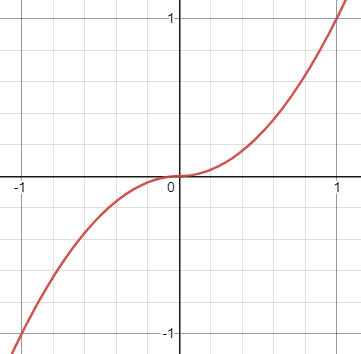
\includegraphics[width=4cm]{pic/tnex2pic1.png}
\anngraphics{4cm}{pic/tnex2pic1.png}{A half-flipped parabola, showing that
it is continuous}
\qquad
%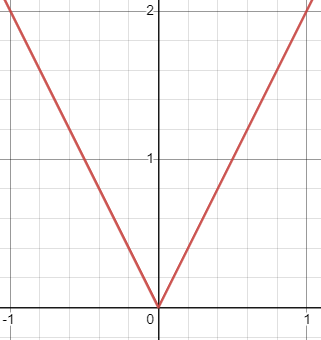
\includegraphics[width=4cm]{pic/tnex2pic2.png}
\anngraphics{4cm}{pic/tnex2pic2.png}{The derivative of this function is
continuous, but not differentiable at x=0}
\end{center}
\caption{A function that is only differentiable once, and its derivative}
\label{tnex2figs}
\end{figure}

The graph of $f$ is formed from a regular parabola except that the left half
has been mirrored across the $x$-axis. Since $f(x) = x^2$ for $x>0$ we know
$f'(x) = 2x$ for $x>0$. Also since $f(x) = -x^2$ for $x<0$ we know $f'(x) =
-2x$ for $x<0$. Using the limit definition of a derivative you can verify
that $f'(0) = 0$ (or just observe from the graph that the tangent line at
$x=0$ is horizontal). Then we can express $f'(x)$ piecewise
\[f'(x) = \begin{cases}
2x & \text{ if }x \geq 0 \\
-2x & \text{ if }x < 0
\end{cases}.\]
Actually there's a simpler way to express $f'(x)$: $f'(x) = 2|x|$. The graph
of this function, Figure~\ref{tnex2figs}, right,
has a ``kink" at $x=0$, which implies that it is not differentiable there.
Of course, it is infinitely differentiable away from $x=0$.
\end{bsp}
Interestingly, this can become far more complicated. There are functions $f(x)$ such that
\begin{itemize}
      \item $f(x)$ is differentiable everywhere ($f'(x)$ exists for all $x$ in the domain of $f$).
      \item $f'(x)$ is continuous everywhere.
      \item $f'(x)$ is not differentiable anywhere in it's domain.
\end{itemize}
However, such functions are extremely unlikely to arise in any practical context,
but just reflect the fact that our definition of a function is rather
general. Indeed, the fact that such functions exist was only established
hundreds of years after the inception of calculus.
